\documentclass[]{book}
\usepackage{lmodern}
\usepackage{amssymb,amsmath}
\usepackage{ifxetex,ifluatex}
\usepackage{fixltx2e} % provides \textsubscript
\ifnum 0\ifxetex 1\fi\ifluatex 1\fi=0 % if pdftex
  \usepackage[T1]{fontenc}
  \usepackage[utf8]{inputenc}
\else % if luatex or xelatex
  \ifxetex
    \usepackage{mathspec}
  \else
    \usepackage{fontspec}
  \fi
  \defaultfontfeatures{Ligatures=TeX,Scale=MatchLowercase}
\fi
% use upquote if available, for straight quotes in verbatim environments
\IfFileExists{upquote.sty}{\usepackage{upquote}}{}
% use microtype if available
\IfFileExists{microtype.sty}{%
\usepackage{microtype}
\UseMicrotypeSet[protrusion]{basicmath} % disable protrusion for tt fonts
}{}
\usepackage[margin=1in]{geometry}
\usepackage{hyperref}
\hypersetup{unicode=true,
            pdftitle={Introduction to Probability and Statistics Using R},
            pdfauthor={G. Jay Kerns},
            pdfborder={0 0 0},
            breaklinks=true}
\urlstyle{same}  % don't use monospace font for urls
\usepackage{biblatex}

\addbibresource{Rpackages.bib}
\addbibresource{IPSUR.bib}
\usepackage{color}
\usepackage{fancyvrb}
\newcommand{\VerbBar}{|}
\newcommand{\VERB}{\Verb[commandchars=\\\{\}]}
\DefineVerbatimEnvironment{Highlighting}{Verbatim}{commandchars=\\\{\}}
% Add ',fontsize=\small' for more characters per line
\usepackage{framed}
\definecolor{shadecolor}{RGB}{248,248,248}
\newenvironment{Shaded}{\begin{snugshade}}{\end{snugshade}}
\newcommand{\KeywordTok}[1]{\textcolor[rgb]{0.13,0.29,0.53}{\textbf{{#1}}}}
\newcommand{\DataTypeTok}[1]{\textcolor[rgb]{0.13,0.29,0.53}{{#1}}}
\newcommand{\DecValTok}[1]{\textcolor[rgb]{0.00,0.00,0.81}{{#1}}}
\newcommand{\BaseNTok}[1]{\textcolor[rgb]{0.00,0.00,0.81}{{#1}}}
\newcommand{\FloatTok}[1]{\textcolor[rgb]{0.00,0.00,0.81}{{#1}}}
\newcommand{\ConstantTok}[1]{\textcolor[rgb]{0.00,0.00,0.00}{{#1}}}
\newcommand{\CharTok}[1]{\textcolor[rgb]{0.31,0.60,0.02}{{#1}}}
\newcommand{\SpecialCharTok}[1]{\textcolor[rgb]{0.00,0.00,0.00}{{#1}}}
\newcommand{\StringTok}[1]{\textcolor[rgb]{0.31,0.60,0.02}{{#1}}}
\newcommand{\VerbatimStringTok}[1]{\textcolor[rgb]{0.31,0.60,0.02}{{#1}}}
\newcommand{\SpecialStringTok}[1]{\textcolor[rgb]{0.31,0.60,0.02}{{#1}}}
\newcommand{\ImportTok}[1]{{#1}}
\newcommand{\CommentTok}[1]{\textcolor[rgb]{0.56,0.35,0.01}{\textit{{#1}}}}
\newcommand{\DocumentationTok}[1]{\textcolor[rgb]{0.56,0.35,0.01}{\textbf{\textit{{#1}}}}}
\newcommand{\AnnotationTok}[1]{\textcolor[rgb]{0.56,0.35,0.01}{\textbf{\textit{{#1}}}}}
\newcommand{\CommentVarTok}[1]{\textcolor[rgb]{0.56,0.35,0.01}{\textbf{\textit{{#1}}}}}
\newcommand{\OtherTok}[1]{\textcolor[rgb]{0.56,0.35,0.01}{{#1}}}
\newcommand{\FunctionTok}[1]{\textcolor[rgb]{0.00,0.00,0.00}{{#1}}}
\newcommand{\VariableTok}[1]{\textcolor[rgb]{0.00,0.00,0.00}{{#1}}}
\newcommand{\ControlFlowTok}[1]{\textcolor[rgb]{0.13,0.29,0.53}{\textbf{{#1}}}}
\newcommand{\OperatorTok}[1]{\textcolor[rgb]{0.81,0.36,0.00}{\textbf{{#1}}}}
\newcommand{\BuiltInTok}[1]{{#1}}
\newcommand{\ExtensionTok}[1]{{#1}}
\newcommand{\PreprocessorTok}[1]{\textcolor[rgb]{0.56,0.35,0.01}{\textit{{#1}}}}
\newcommand{\AttributeTok}[1]{\textcolor[rgb]{0.77,0.63,0.00}{{#1}}}
\newcommand{\RegionMarkerTok}[1]{{#1}}
\newcommand{\InformationTok}[1]{\textcolor[rgb]{0.56,0.35,0.01}{\textbf{\textit{{#1}}}}}
\newcommand{\WarningTok}[1]{\textcolor[rgb]{0.56,0.35,0.01}{\textbf{\textit{{#1}}}}}
\newcommand{\AlertTok}[1]{\textcolor[rgb]{0.94,0.16,0.16}{{#1}}}
\newcommand{\ErrorTok}[1]{\textcolor[rgb]{0.64,0.00,0.00}{\textbf{{#1}}}}
\newcommand{\NormalTok}[1]{{#1}}
\usepackage{longtable,booktabs}
\usepackage{graphicx,grffile}
\makeatletter
\def\maxwidth{\ifdim\Gin@nat@width>\linewidth\linewidth\else\Gin@nat@width\fi}
\def\maxheight{\ifdim\Gin@nat@height>\textheight\textheight\else\Gin@nat@height\fi}
\makeatother
% Scale images if necessary, so that they will not overflow the page
% margins by default, and it is still possible to overwrite the defaults
% using explicit options in \includegraphics[width, height, ...]{}
\setkeys{Gin}{width=\maxwidth,height=\maxheight,keepaspectratio}
\IfFileExists{parskip.sty}{%
\usepackage{parskip}
}{% else
\setlength{\parindent}{0pt}
\setlength{\parskip}{6pt plus 2pt minus 1pt}
}
\setlength{\emergencystretch}{3em}  % prevent overfull lines
\providecommand{\tightlist}{%
  \setlength{\itemsep}{0pt}\setlength{\parskip}{0pt}}
\setcounter{secnumdepth}{5}
% Redefines (sub)paragraphs to behave more like sections
\ifx\paragraph\undefined\else
\let\oldparagraph\paragraph
\renewcommand{\paragraph}[1]{\oldparagraph{#1}\mbox{}}
\fi
\ifx\subparagraph\undefined\else
\let\oldsubparagraph\subparagraph
\renewcommand{\subparagraph}[1]{\oldsubparagraph{#1}\mbox{}}
\fi

%%% Use protect on footnotes to avoid problems with footnotes in titles
\let\rmarkdownfootnote\footnote%
\def\footnote{\protect\rmarkdownfootnote}

%%% Change title format to be more compact
\usepackage{titling}

% Create subtitle command for use in maketitle
\newcommand{\subtitle}[1]{
  \posttitle{
    \begin{center}\large#1\end{center}
    }
}

\setlength{\droptitle}{-2em}
  \title{Introduction to Probability and Statistics Using R}
  \pretitle{\vspace{\droptitle}\centering\huge}
  \posttitle{\par}
  \author{G. Jay Kerns}
  \preauthor{\centering\large\emph}
  \postauthor{\par}
  \predate{\centering\large\emph}
  \postdate{\par}
  \date{2017-02-03}

%    IPSUR: Introduction to Probability and Statistics Using R
%    Copyright (C)  2017 G. Jay Kerns
%
%    This file is part of IPSUR.
%
%    Permission is granted to copy, distribute and/or modify this document
%    under the terms of the GNU Free Documentation License, Version 1.3
%    or any later version published by the Free Software Foundation;
%    with no Invariant Sections, no Front-Cover Texts, and no Back-Cover Texts.
%    A copy of the license is contained in the LICENSE file in this 
%    directory.

\subtitle{Third Edition}

\usepackage{lmodern}
\renewcommand{\sfdefault}{lmss}
\renewcommand{\ttdefault}{lmtt}

% needed packages
\usepackage{amsmath}
\usepackage{amssymb}
\usepackage{amsthm}
\usepackage[english]{babel}
\usepackage{epsfig}
\usepackage{fancyvrb}
\usepackage{fixltx2e}
\usepackage{float}
%\usepackage{floatflt}
\usepackage[T1]{fontenc}
\usepackage{footnote}
%\usepackage{graphics}
\usepackage{graphicx}
\usepackage[utf8]{inputenc}
\usepackage{latexsym}
\usepackage{longtable}
\usepackage{makeidx}
\usepackage{marvosym}
\usepackage{multicol}
%\usepackage{pslatex}
%\usepackage{showidx}
\usepackage{soul}
\usepackage{srcltx}
\usepackage{stmaryrd}
\usepackage{subfig}
\usepackage{textcomp}
%\usepackage{theorem}
\usepackage[subfigure]{tocloft}
\usepackage{txfonts}
\usepackage{upgreek}
\usepackage{url}
\usepackage{varioref}
\usepackage{verbatim}
%\usepackage{wasysym}
\usepackage{wrapfig}

% Page setup
%\usepackage[paperwidth=7.44in,paperheight=9.69in]{geometry}
%\geometry{verbose,tmargin=1in,bmargin=1in,outer=1.25in,inner=0.75in}
\geometry{paperwidth=7.44in,paperheight=9.69in}
\pagestyle{headings}
\setcounter{secnumdepth}{2}
\setcounter{tocdepth}{1}


\makeindex


% PDF settings
\usepackage[hyperref,x11names]{xcolor}
\usepackage{hyperref}
\hypersetup{pdftitle={Introduction to Probability and Statistics Using R},
 		pdfauthor={G. Jay Kerns}, 
		linkcolor=Firebrick4, 
		citecolor=black, 
		urlcolor=SteelBlue4}

% special logos
\providecommand{\IPSUR}
{\textsc{I\kern 0ex\lower-0.3ex\hbox{\small P}\kern -0.5ex\lower0.4ex\hbox{\footnotesize S}\kern -0.25exU}\kern -0.1ex\lower 0.15ex\hbox{\textsf{\large R}}\@}

%  user defined commands
% special operators

\renewcommand{\vec}[1]{\mbox{\boldmath$#1$}}

\makeatletter


%%%%%%%%%%%%%%%%%%%%%%%%%%%%%% Textclass specific LaTeX commands.

\numberwithin{equation}{chapter}
\numberwithin{figure}{chapter}

\theoremstyle{plain}
  \newtheorem{thm}{Theorem}[chapter]
  \newtheorem{fact}[thm]{Fact}
  \newtheorem{ax}[thm]{Axiom}
  \newtheorem{prop}[thm]{Proposition}
  \newtheorem{cor}[thm]{Corollary}
  \newtheorem{assumption}[thm]{Assumption}

\theoremstyle{definition}
  \newtheorem{defn}[thm]{Definition}
  \newtheorem{example}[thm]{Example}
  \newtheorem{xca}{Exercise}[chapter]

\theoremstyle{remark}
  \newtheorem{note}[thm]{Note}
  \newtheorem{rem}[thm]{Remark}

\setlength{\cftfignumwidth}{1.5cm}

\@ifundefined{showcaptionsetup}{}{%
 \PassOptionsToPackage{caption=false}{subfig}}
\usepackage{subfig}
\AtBeginDocument{
  \def\labelitemii{\(\circ\)}
}

\makeatother

\let\BeginKnitrBlock\begin \let\EndKnitrBlock\end
\begin{document}
\maketitle

{
\setcounter{tocdepth}{1}
\tableofcontents
}
\chapter{An Introduction to Probability and
Statistics}\label{cha-introps}

This chapter has proved to be the hardest to write, by far. The trouble
is that there is so much to say -- and so many people have already said
it so much better than I could. When I get something I like I will
release it here.

In the meantime, there is a lot of information already available to a
person with an Internet connection. I recommend to start at Wikipedia,
which is not a flawless resource but it has the main ideas with links to
reputable sources.

In my lectures I usually tell stories about Fisher, Galton, Gauss,
Laplace, Quetelet, and the Chevalier de Mere.

\section{Probability}\label{probability}

The common folklore is that probability has been around for millennia
but did not gain the attention of mathematicians until approximately
1654 when the Chevalier de Mere had a question regarding the fair
division of a game's payoff to the two players, supposing the game had
to end prematurely.

\section{Statistics}\label{statistics}

Statistics concerns data; their collection, analysis, and
interpretation. In this book we distinguish between two types of
statistics: descriptive and inferential.

Descriptive statistics concerns the summarization of data. We have a
data set and we would like to describe the data set in multiple ways.
Usually this entails calculating numbers from the data, called
descriptive measures, such as percentages, sums, averages, and so forth.

Inferential statistics does more. There is an inference associated with
the data set, a conclusion drawn about the population from which the
data originated.

I would like to mention that there are two schools of thought of
statistics: frequentist and bayesian. The difference between the schools
is related to how the two groups interpret the underlying probability
(see Section \{\#sec-interpreting-probabilities\}). The frequentist
school gained a lot of ground among statisticians due in large part to
the work of Fisher, Neyman, and Pearson in the early twentieth century.
That dominance lasted until inexpensive computing power became widely
available; nowadays the bayesian school is garnering more attention and
at an increasing rate.

This book is devoted mostly to the frequentist viewpoint because that is
how I was trained, with the conspicuous exception of Sections
\{\#sec-bayes-rule\} and \{\#sec-conditional-distributions\}. I plan to
add more bayesian material in later editions of this book.
\ref{fig:stripcharts}

\chapter{An Introduction to R}\label{cha-introduction-to-R}

Every R book I have ever seen has had a section/chapter that is an
introduction to R, and so does this one. The goal of this chapter is for
a person to get up and running, ready for the material that follows. See
Section \ref{sec-External-Resources} for links to other material which
the reader may find useful.

\textbf{What do I want them to know?}

\begin{itemize}
\tightlist
\item
  Where to find R to install on a home computer, and a few comments to
  help with the usual hiccups that occur when installing something.
\item
  Abbreviated remarks about the available options to interact with R.
\item
  Basic operations (arithmetic, entering data, vectors) at the command
  prompt.
\item
  How and where to find help when they get in trouble.
\item
  Other little shortcuts I am usually asked when introducing R.
\end{itemize}

\section{Downloading and Installing R}\label{sec-download-install-R}

The instructions for obtaining R largely depend on the user's hardware
and operating system. The R Project has written an R Installation and
Administration manual with complete, precise instructions about what to
do, together with all sorts of additional information. The following is
just a primer to get a person started.

\subsection{Installing R}\label{installing-r}

Visit one of the links below to download the latest version of R for
your operating system:

\begin{itemize}
\tightlist
\item
  Microsoft Windows: \url{http://cran.r-project.org/bin/windows/base/}
\item
  MacOS: \url{http://cran.r-project.org/bin/macosx/}
\item
  Linux: \url{http://cran.r-project.org/bin/linux/}
\end{itemize}

On Microsoft Windows, click the \texttt{R-x.y.z.exe} installer to start
installation. When it asks for ``Customized startup options'', specify
\texttt{Yes}. In the next window, be sure to select the SDI (single
document interface) option; this is useful later when we discuss three
dimensional plots with the \texttt{rgl} package \autocite{rgl}.

\subsubsection{Installing R on a USB drive
(Windows)}\label{installing-r-on-a-usb-drive-windows}

With this option you can use R portably and without administrative
privileges. There is an entry in the R for Windows FAQ about this. Here
is the procedure I use:

\begin{enumerate}
\def\labelenumi{\arabic{enumi}.}
\tightlist
\item
  Download the Windows installer above and start installation as usual.
  When it asks \emph{where} to install, navigate to the top-level
  directory of the USB drive instead of the default \texttt{C} drive.
\item
  When it asks whether to modify the Windows registry, uncheck the box;
  we do NOT want to tamper with the registry.
\item
  After installation, change the name of the folder from
  \texttt{R-x.y.z} to just plain R. (Even quicker: do this in step 1.)
\item
  \href{http://ipsur.r-forge.r-project.org/book/download/R.exe}{Download
  this shortcut} and move it to the top-level directory of the USB
  drive, right beside the R folder, not inside the folder. Use the
  downloaded shortcut to run R.
\end{enumerate}

Steps 3 and 4 are not required but save you the trouble of navigating to
the \texttt{R-x.y.z/bin} directory to double-click \texttt{Rgui.exe}
every time you want to run the program. It is useless to create your own
shortcut to \texttt{Rgui.exe}. Windows does not allow shortcuts to have
relative paths; they always have a drive letter associated with them. So
if you make your own shortcut and plug your USB drive into some
\emph{other} machine that happens to assign your drive a different
letter, then your shortcut will no longer be pointing to the right
place.

\subsection{Installing and Loading Add-on
Packages}\label{sub-installing-loading-packages}

There are \emph{base} packages (which come with R automatically), and
\emph{contributed} packages (which must be downloaded for installation).
For example, on the version of R being used for this document the
default base packages loaded at startup are

\begin{Shaded}
\begin{Highlighting}[]
\KeywordTok{getOption}\NormalTok{(}\StringTok{"defaultPackages"}\NormalTok{)}
\end{Highlighting}
\end{Shaded}

\begin{verbatim}
## [1] "datasets"  "utils"     "grDevices" "graphics"  "stats"     "methods"
\end{verbatim}

The base packages are maintained by a select group of volunteers, called
R Core. In addition to the base packages, there are over ten thousand
additional contributed packages written by individuals all over the
world. These are stored worldwide on mirrors of the Comprehensive R
Archive Network, or \texttt{CRAN} for short. Given an active Internet
connection, anybody is free to download and install these packages and
even inspect the source code.

To install a package named \texttt{foo}, open up R and type
\texttt{install.packages("foo")}
\index{install.packages@\texttt{install.packages}}. To install
\texttt{foo} and additionally install all of the other packages on which
\texttt{foo} depends, instead type
\texttt{install.packages("foo",\ depends\ =\ TRUE)}.

The general command \texttt{install.packages()} will (on most operating
systems) open a window containing a huge list of available packages;
simply choose one or more to install.

No matter how many packages are installed onto the system, each one must
first be loaded for use with the \texttt{library}
\index{library@\texttt{library}} function. For instance, the
\texttt{foreign} package \autocite{foreign} contains all sorts of
functions needed to import data sets into R from other software such as
SPSS, SAS, \emph{etc}. But none of those functions will be available
until the command \texttt{library("foreign")} is issued.

Type \texttt{library()} at the command prompt (described below) to see a
list of all available packages in your library.

For complete, precise information regarding installation of R and add-on
packages, see the \href{http://cran.r-project.org/manuals.html}{R
Installation and Administration manual}.

\section{Communicating with R}\label{sec-Communicating-with-R}

\subsection{One line at a time}\label{one-line-at-a-time}

This is the most basic method and is the first one that beginners will
use.

\begin{itemize}
\tightlist
\item
  RGui (Microsoft \(\circledR\) Windows)
\item
  RStudio
\item
  Terminal
\item
  Emacs/ESS, XEmacs
\end{itemize}

\subsection{Multiple lines at a time}\label{multiple-lines-at-a-time}

For longer programs (called \emph{scripts}) there is too much code to
write all at once at the command prompt. Furthermore, for longer scripts
it is convenient to be able to only modify a certain piece of the script
and run it again in R. Programs called \emph{script editors} are
specially designed to aid the communication and code writing process.
They have all sorts of helpful features including R syntax highlighting,
automatic code completion, delimiter matching, and dynamic help on the R
functions as they are being written. Even more, they often have all of
the text editing features of programs like Microsoft\(\circledR\)Word.
Lastly, most script editors are fully customizable in the sense that the
user can customize the appearance of the interface to choose what colors
to display, when to display them, and how to display them.

\begin{itemize}
\tightlist
\item
  \textbf{R Editor (Windows):} In Microsoft\(\circledR\) Windows, R Gui
  has its own built-in script editor, called R Editor. From the console
  window, select \texttt{File} \(\triangleright\) \texttt{New\ Script}.
  A script window opens, and the lines of code can be written in the
  window. When satisfied with the code, the user highlights all of the
  commands and presses \textsf{Ctrl+R}. The commands are automatically
  run at once in R and the output is shown. To save the script for
  later, click \texttt{File} \(\triangleright\) \texttt{Save\ as...} in
  R Editor. The script can be reopened later with \texttt{File}
  \(\triangleright\)\} \texttt{Open\ Script...} in \texttt{RGui}. Note
  that R Editor does not have the fancy syntax highlighting that the
  others do.
\item
  \textbf{RStudio:}
\item
  \textbf{Emacs/ESS:} Emacs is an all purpose text editor. It can do
  absolutely anything with respect to modifying, searching, editing, and
  manipulating, text. And if Emacs can't do it, then you can write a
  program that extends Emacs to do it. Once such extension is called
  \texttt{ESS}, which stands for /E/-macs /S/-peaks /S/-tatistics. With
  ESS a person can speak to R, do all of the tricks that the other
  script editors offer, and much, much, more. Please see the following
  for installation details, documentation, reference cards, and a whole
  lot more: \url{http://ess.r-project.org}. \emph{Fair warning}: if you
  want to try Emacs and if you grew up with Microsoft\(\circledR\)
  Windows or Macintosh, then you are going to need to relearn everything
  you thought you knew about computers your whole life. (Or, since Emacs
  is completely customizable, you can reconfigure Emacs to behave the
  way you want.) I have personally experienced this transformation and I
  will never go back.
\end{itemize}

\subsection{Graphical User Interfaces
(GUIs)}\label{graphical-user-interfaces-guis}

By the word ``GUI'' I mean an interface in which the user communicates
with R by way of points-and-clicks in a menu of some sort. Again, there
are many, many options and I only mention one that I have used and
enjoyed.

\begin{itemize}
\tightlist
\item
  \textbf{R Commander} provides a point-and-click interface to many
  basic statistical tasks. It is called the ``Commander'' because every
  time one makes a selection from the menus, the code corresponding to
  the task is listed in the output window. One can take this code,
  copy-and-paste it to a text file, then re-run it again at a later time
  without the R Commander's assistance. It is well suited for the
  introductory level. \texttt{Rcmdr} \autocite{Rcmdr} also allows for
  user-contributed ``Plugins'' which are separate packages on
  \texttt{CRAN} that add extra functionality to the \texttt{Rcmdr}
  package. The plugins are typically named with the prefix
  \texttt{RcmdrPlugin} to make them easy to identify in the
  \texttt{CRAN} package list. One such plugin is the
  \texttt{RcmdrPlugin.IPSUR} package \autocite{RcmdrPlugin.IPSUR} which
  accompanies this text.
\end{itemize}

\section{Basic R Operations and Concepts}\label{sec-Basic-R-Operations}

The R developers have written an introductory document entitled ``An
Introduction to R''. There is a sample session included which shows what
basic interaction with R looks like. I recommend that all new users of R
read that document, but bear in mind that there are concepts mentioned
which will be unfamiliar to the beginner.

Below are some of the most basic operations that can be done with R.
Almost every book about R begins with a section like the one below; look
around to see all sorts of things that can be done at this most basic
level.

\subsection{Arithmetic}\label{sub-Arithmetic}

\begin{Shaded}
\begin{Highlighting}[]
\DecValTok{2} \NormalTok{+}\StringTok{ }\DecValTok{3}       \CommentTok{# add}
\end{Highlighting}
\end{Shaded}

\begin{verbatim}
## [1] 5
\end{verbatim}

\begin{Shaded}
\begin{Highlighting}[]
\DecValTok{4} \CommentTok{# 5 / 6   # multiply and divide}
\end{Highlighting}
\end{Shaded}

\begin{verbatim}
## [1] 4
\end{verbatim}

\begin{Shaded}
\begin{Highlighting}[]
\DecValTok{7}\NormalTok{^}\DecValTok{8}         \CommentTok{# 7 to the 8th power}
\end{Highlighting}
\end{Shaded}

\begin{verbatim}
## [1] 5764801
\end{verbatim}

Notice the comment character \texttt{\#}. Anything typed after a
\texttt{\#} symbol is ignored by R. We know that \(20/6\) is a repeating
decimal, but the above example shows only 7 digits. We can change the
number of digits displayed with \texttt{options}:

\begin{Shaded}
\begin{Highlighting}[]
\KeywordTok{options}\NormalTok{(}\DataTypeTok{digits =} \DecValTok{16}\NormalTok{)}
\DecValTok{10}\NormalTok{/}\DecValTok{3}                 \CommentTok{# see more digits}
\end{Highlighting}
\end{Shaded}

\begin{verbatim}
## [1] 3.333333333333333
\end{verbatim}

\begin{Shaded}
\begin{Highlighting}[]
\KeywordTok{sqrt}\NormalTok{(}\DecValTok{2}\NormalTok{)              }\CommentTok{# square root}
\end{Highlighting}
\end{Shaded}

\begin{verbatim}
## [1] 1.414213562373095
\end{verbatim}

\begin{Shaded}
\begin{Highlighting}[]
\KeywordTok{exp}\NormalTok{(}\DecValTok{1}\NormalTok{)               }\CommentTok{# Euler's constant, e}
\end{Highlighting}
\end{Shaded}

\begin{verbatim}
## [1] 2.718281828459045
\end{verbatim}

\begin{Shaded}
\begin{Highlighting}[]
\NormalTok{pi       }
\end{Highlighting}
\end{Shaded}

\begin{verbatim}
## [1] 3.141592653589793
\end{verbatim}

\begin{Shaded}
\begin{Highlighting}[]
\KeywordTok{options}\NormalTok{(}\DataTypeTok{digits =} \DecValTok{7}\NormalTok{)  }\CommentTok{# back to default}
\end{Highlighting}
\end{Shaded}

Note that it is possible to set \texttt{digits} up to 22, but setting
them over 16 is not recommended (the extra significant digits are not
necessarily reliable). Above notice the \texttt{sqrt} function for
square roots and the \texttt{exp} \index{exp@\texttt{exp}} function for
powers of \(\mathrm{e}\), Euler's number.

\subsection{Assignment, Object names, and Data
types}\label{sub-Assignment-Object-names}

It is often convenient to assign numbers and values to variables
(objects) to be used later. The proper way to assign values to a
variable is with the \texttt{\textless{}-} operator (with a space on
either side). The \texttt{=} symbol works too, but it is recommended by
the R masters to reserve \texttt{=} for specifying arguments to
functions (discussed later). In this book we will follow their advice
and use \texttt{\textless{}-} for assignment. Once a variable is
assigned, its value can be printed by simply entering the variable name
by itself.

\begin{Shaded}
\begin{Highlighting}[]
\NormalTok{x <-}\StringTok{ }\DecValTok{7}\NormalTok{*}\DecValTok{41}\NormalTok{/pi   }\CommentTok{# don't see the calculated value}
\NormalTok{x              }\CommentTok{# take a look}
\end{Highlighting}
\end{Shaded}

\begin{verbatim}
## [1] 91.35494
\end{verbatim}

When choosing a variable name you can use letters, numbers, dots
``\texttt{.}'', or underscore ``\texttt{\_}'' characters. You cannot use
mathematical operators, and a leading dot may not be followed by a
number. Examples of valid names are: \texttt{x}, \texttt{x1},
\texttt{y.value}, and \texttt{!y\_hat}. (More precisely, the set of
allowable characters in object names depends on one's particular system
and locale; see An Introduction to R for more discussion on this.)

Objects can be of many \emph{types}, \emph{modes}, and \emph{classes}.
At this level, it is not necessary to investigate all of the intricacies
of the respective types, but there are some with which you need to
become familiar: * integer: the values \(0\), \(\pm1\), \(\pm2\),
\ldots{}; these are represented exactly by R. * double: real numbers
(rational and irrational); these numbers are not represented exactly
(save integers or fractions with a denominator that is a power of 2, see
\textcite{Venables2010} ). * character: elements that are wrapped with
pairs of \texttt{"} or '; * logical: includes \texttt{TRUE},
\texttt{FALSE}, and \texttt{NA} (which are reserved words); the
\texttt{NA} \index{NA@\texttt{NA}} stands for ``not available'',
\emph{i.e.}, a missing value.

You can determine an object's type with the \texttt{typeof}
\index{typeof@\texttt{typeof}} function. In addition to the above, there
is the \texttt{complex} \index{complex@\texttt{complex}}
\index{as.complex@\texttt{as.complex}} data type:

\begin{Shaded}
\begin{Highlighting}[]
\KeywordTok{sqrt}\NormalTok{(-}\DecValTok{1}\NormalTok{)              }\CommentTok{# isn't defined}
\end{Highlighting}
\end{Shaded}

\begin{verbatim}
## Warning in sqrt(-1): NaNs produced
\end{verbatim}

\begin{verbatim}
## [1] NaN
\end{verbatim}

\begin{Shaded}
\begin{Highlighting}[]
\KeywordTok{sqrt}\NormalTok{(-}\DecValTok{1}\NormalTok{+0i)           }\CommentTok{# is defined}
\end{Highlighting}
\end{Shaded}

\begin{verbatim}
## [1] 0+1i
\end{verbatim}

\begin{Shaded}
\begin{Highlighting}[]
\KeywordTok{sqrt}\NormalTok{(}\KeywordTok{as.complex}\NormalTok{(-}\DecValTok{1}\NormalTok{))  }\CommentTok{# same thing}
\end{Highlighting}
\end{Shaded}

\begin{verbatim}
## [1] 0+1i
\end{verbatim}

\begin{Shaded}
\begin{Highlighting}[]
\NormalTok{(}\DecValTok{0} \NormalTok{+}\StringTok{ }\NormalTok{1i)^}\DecValTok{2}            \CommentTok{# should be -1}
\end{Highlighting}
\end{Shaded}

\begin{verbatim}
## [1] -1+0i
\end{verbatim}

\begin{Shaded}
\begin{Highlighting}[]
\KeywordTok{typeof}\NormalTok{((}\DecValTok{0} \NormalTok{+}\StringTok{ }\NormalTok{1i)^}\DecValTok{2}\NormalTok{)}
\end{Highlighting}
\end{Shaded}

\begin{verbatim}
## [1] "complex"
\end{verbatim}

Note that you can just type \texttt{(1i)\^{}2} to get the same answer.
The \texttt{NaN} \index{NaN@\texttt{NaN}} stands for ``not a number'';
it is represented internally as \texttt{double} \index{double}.

\subsection{Vectors}\label{vectors}

:PROPERTIES: :CUSTOM\_ID: sub-Vectors :END:

All of this time we have been manipulating vectors of length 1. Now let
us move to vectors with multiple entries.

\subsubsection{Entering data vectors}\label{entering-data-vectors}

\textbf{The long way:} \index{c@\texttt{c}} If you would like to enter
the data \texttt{74,31,95,61,76,34,23,54,96} into R, you may create a
data vector with the \texttt{c} function (which is short for
\emph{concatenate}).

\begin{Shaded}
\begin{Highlighting}[]
\NormalTok{x <-}\StringTok{ }\KeywordTok{c}\NormalTok{(}\DecValTok{74}\NormalTok{, }\DecValTok{31}\NormalTok{, }\DecValTok{95}\NormalTok{, }\DecValTok{61}\NormalTok{, }\DecValTok{76}\NormalTok{, }\DecValTok{34}\NormalTok{, }\DecValTok{23}\NormalTok{, }\DecValTok{54}\NormalTok{, }\DecValTok{96}\NormalTok{)}
\NormalTok{x}
\end{Highlighting}
\end{Shaded}

\begin{verbatim}
## [1] 74 31 95 61 76 34 23 54 96
\end{verbatim}

The elements of a vector are usually coerced by R to the the most
general type of any of the elements, so if you do \texttt{c(1,\ "2")}
then the result will be \texttt{c("1",\ "2")}.

\textbf{A shorter way:} \index{scan@\texttt{scan}}: The \texttt{scan}
method is useful when the data are stored somewhere else. For instance,
you may type \texttt{x\ \textless{}-\ scan()} at the command prompt and
R will display \texttt{1:} to indicate that it is waiting for the first
data value. Type a value and press \texttt{Enter}, at which point R will
display \texttt{2:}, and so forth. Note that entering an empty line
stops the scan. This method is especially handy when you have a column
of values, say, stored in a text file or spreadsheet. You may copy and
paste them all at the \texttt{1:} prompt, and R will store all of the
values instantly in the vector \texttt{x}.

*Repeated data; regular patterns:\# the \texttt{seq}
\index{seq@\texttt{seq}} function will generate all sorts of sequences
of numbers. It has the arguments \texttt{from}, \texttt{to},
\texttt{by}, and \texttt{length.out} which can be set in concert with
one another. We will do a couple of examples to show you how it works.

\begin{Shaded}
\begin{Highlighting}[]
\KeywordTok{seq}\NormalTok{(}\DataTypeTok{from =} \DecValTok{1}\NormalTok{, }\DataTypeTok{to =} \DecValTok{5}\NormalTok{)}
\end{Highlighting}
\end{Shaded}

\begin{verbatim}
## [1] 1 2 3 4 5
\end{verbatim}

\begin{Shaded}
\begin{Highlighting}[]
\KeywordTok{seq}\NormalTok{(}\DataTypeTok{from =} \DecValTok{2}\NormalTok{, }\DataTypeTok{by =} \NormalTok{-}\FloatTok{0.1}\NormalTok{, }\DataTypeTok{length.out =} \DecValTok{4}\NormalTok{)}
\end{Highlighting}
\end{Shaded}

\begin{verbatim}
## [1] 2.0 1.9 1.8 1.7
\end{verbatim}

Note that we can get the first line much quicker with the colon
operator.

\begin{Shaded}
\begin{Highlighting}[]
\DecValTok{1}\NormalTok{:}\DecValTok{5}
\end{Highlighting}
\end{Shaded}

\begin{verbatim}
## [1] 1 2 3 4 5
\end{verbatim}

The vector \texttt{LETTERS} \index{LETTERS@\texttt{LETTERS}} has the 26
letters of the English alphabet in uppercase and \texttt{letters}
\index{letters@\texttt{letters}} has all of them in lowercase.

\subsubsection{Indexing data vectors}\label{indexing-data-vectors}

Sometimes we do not want the whole vector, but just a piece of it. We
can access the intermediate parts with the \texttt{{[}{]}} operator.
Observe (with \texttt{x} defined above)

\begin{Shaded}
\begin{Highlighting}[]
\NormalTok{x[}\DecValTok{1}\NormalTok{]}
\end{Highlighting}
\end{Shaded}

\begin{verbatim}
## [1] 74
\end{verbatim}

\begin{Shaded}
\begin{Highlighting}[]
\NormalTok{x[}\DecValTok{2}\NormalTok{:}\DecValTok{4}\NormalTok{]}
\end{Highlighting}
\end{Shaded}

\begin{verbatim}
## [1] 31 95 61
\end{verbatim}

\begin{Shaded}
\begin{Highlighting}[]
\NormalTok{x[}\KeywordTok{c}\NormalTok{(}\DecValTok{1}\NormalTok{,}\DecValTok{3}\NormalTok{,}\DecValTok{4}\NormalTok{,}\DecValTok{8}\NormalTok{)]}
\end{Highlighting}
\end{Shaded}

\begin{verbatim}
## [1] 74 95 61 54
\end{verbatim}

\begin{Shaded}
\begin{Highlighting}[]
\NormalTok{x[-}\KeywordTok{c}\NormalTok{(}\DecValTok{1}\NormalTok{,}\DecValTok{3}\NormalTok{,}\DecValTok{4}\NormalTok{,}\DecValTok{8}\NormalTok{)]}
\end{Highlighting}
\end{Shaded}

\begin{verbatim}
## [1] 31 76 34 23 96
\end{verbatim}

Notice that we used the minus sign to specify those elements that we do
\emph{not} want.

\begin{Shaded}
\begin{Highlighting}[]
\NormalTok{LETTERS[}\DecValTok{1}\NormalTok{:}\DecValTok{5}\NormalTok{]}
\end{Highlighting}
\end{Shaded}

\begin{verbatim}
## [1] "A" "B" "C" "D" "E"
\end{verbatim}

\begin{Shaded}
\begin{Highlighting}[]
\NormalTok{letters[-(}\DecValTok{6}\NormalTok{:}\DecValTok{24}\NormalTok{)]}
\end{Highlighting}
\end{Shaded}

\begin{verbatim}
## [1] "a" "b" "c" "d" "e" "y" "z"
\end{verbatim}

\subsection{Functions and
Expressions}\label{sub-Functions-and-Expressions}

A function takes arguments as input and returns an object as output.
There are functions to do all sorts of things. We show some examples
below.

\begin{Shaded}
\begin{Highlighting}[]
\NormalTok{x <-}\StringTok{ }\DecValTok{1}\NormalTok{:}\DecValTok{5}
\KeywordTok{sum}\NormalTok{(x)}
\end{Highlighting}
\end{Shaded}

\begin{verbatim}
## [1] 15
\end{verbatim}

\begin{Shaded}
\begin{Highlighting}[]
\KeywordTok{length}\NormalTok{(x)}
\end{Highlighting}
\end{Shaded}

\begin{verbatim}
## [1] 5
\end{verbatim}

\begin{Shaded}
\begin{Highlighting}[]
\KeywordTok{min}\NormalTok{(x)}
\end{Highlighting}
\end{Shaded}

\begin{verbatim}
## [1] 1
\end{verbatim}

\begin{Shaded}
\begin{Highlighting}[]
\KeywordTok{mean}\NormalTok{(x)      }\CommentTok{# sample mean}
\end{Highlighting}
\end{Shaded}

\begin{verbatim}
## [1] 3
\end{verbatim}

\begin{Shaded}
\begin{Highlighting}[]
\KeywordTok{sd}\NormalTok{(x)        }\CommentTok{# sample standard deviation}
\end{Highlighting}
\end{Shaded}

\begin{verbatim}
## [1] 1.581139
\end{verbatim}

It will not be long before the user starts to wonder how a particular
function is doing its job, and since R is open-source, anybody is free
to look under the hood of a function to see how things are calculated.
For detailed instructions see the article ``Accessing the Sources'' by
Uwe Ligges \autocite{Ligges2006}. In short:

\textbf{Type the name of the function} without any parentheses or
arguments. If you are lucky then the code for the entire function will
be printed, right there looking at you. For instance, suppose that we
would like to see how the \texttt{intersect}
\index{intersect@\texttt{intersect}} function works:

\begin{Shaded}
\begin{Highlighting}[]
\NormalTok{intersect}
\end{Highlighting}
\end{Shaded}

\begin{verbatim}
## function (x, y) 
## {
##     y <- as.vector(y)
##     unique(y[match(as.vector(x), y, 0L)])
## }
## <bytecode: 0x349a230>
## <environment: namespace:base>
\end{verbatim}

If instead it shows \texttt{UseMethod(something)}
\index{UseMethod@\texttt{UseMethod}} then you will need to choose the
\emph{class} of the object to be inputted and next look at the
\emph{method} that will be \emph{dispatched} to the object. For
instance, typing \texttt{rev} \index{rev@\texttt{rev}} says

\begin{Shaded}
\begin{Highlighting}[]
\NormalTok{rev}
\end{Highlighting}
\end{Shaded}

\begin{verbatim}
## function (x) 
## UseMethod("rev")
## <bytecode: 0x2bfce40>
## <environment: namespace:base>
\end{verbatim}

The output is telling us that there are multiple methods associated with
the \texttt{rev} function. To see what these are, type

\begin{Shaded}
\begin{Highlighting}[]
\KeywordTok{methods}\NormalTok{(rev)}
\end{Highlighting}
\end{Shaded}

\begin{verbatim}
## [1] rev.default     rev.dendrogram*
## see '?methods' for accessing help and source code
\end{verbatim}

Now we learn that there are two different \texttt{rev(x)} functions,
only one of which being chosen at each call depending on what \texttt{x}
is. There is one for \texttt{dendrogram} objects and a \texttt{default}
method for everything else. Simply type the name to see what each method
does. For example, the \texttt{default} method can be viewed with

\begin{Shaded}
\begin{Highlighting}[]
\NormalTok{rev.default}
\end{Highlighting}
\end{Shaded}

\begin{verbatim}
## function (x) 
## if (length(x)) x[length(x):1L] else x
## <bytecode: 0x3125768>
## <environment: namespace:base>
\end{verbatim}

\textbf{Some functions are hidden by a namespace} (see An Introduction
to R \textcite{Venables2010}), and are not visible on the first try. For
example, if we try to look at the code for \texttt{wilcox.test}
\index{wilcox.test@\texttt{wilcox.test}} (see Chapter
\ref{cha-Nonparametric-Statistics}) we get the following:

\begin{Shaded}
\begin{Highlighting}[]
\NormalTok{wilcox.test}
\end{Highlighting}
\end{Shaded}

\begin{verbatim}
## function (x, ...) 
## UseMethod("wilcox.test")
## <bytecode: 0x2adadf0>
## <environment: namespace:stats>
\end{verbatim}

\begin{Shaded}
\begin{Highlighting}[]
\KeywordTok{methods}\NormalTok{(wilcox.test)}
\end{Highlighting}
\end{Shaded}

\begin{verbatim}
## [1] wilcox.test.default* wilcox.test.formula*
## see '?methods' for accessing help and source code
\end{verbatim}

If we were to try \texttt{wilcox.test.default} we would get a ``not
found'' error, because it is hidden behind the namespace for the package
\texttt{stats} \autocite{stats} (shown in the last line when we tried
\texttt{wilcox.test}). In cases like these we prefix the package name to
the front of the function name with three colons; the command
\texttt{stats:::wilcox.test.default} will show the source code, omitted
here for brevity.

If it shows \texttt{.Internal(something)}
\index{.Internal@\texttt{.Internal}} or \texttt{.Primitive(something)}
\index{.Primitive@\texttt{.Primitive}}, then it will be necessary to
download the source code of R (which is \emph{not} a binary version with
an \texttt{.exe} extension) and search inside the code there. See Ligges
\autocite{Ligges2006} for more discussion on this. An example is
\texttt{exp}:

\begin{Shaded}
\begin{Highlighting}[]
\NormalTok{exp}
\end{Highlighting}
\end{Shaded}

\begin{verbatim}
## function (x)  .Primitive("exp")
\end{verbatim}

Be warned that most of the \texttt{.Internal} functions are written in
other computer languages which the beginner may not understand, at least
initially.

\section{Getting Help}\label{sec-getting-help}

When you are using R, it will not take long before you find yourself
needing help. Fortunately, R has extensive help resources and you should
immediately become familiar with them. Begin by clicking \texttt{Help}
on \texttt{RGui}. The following options are available.

\begin{itemize}
\tightlist
\item
  Console: gives useful shortcuts, for instance, \texttt{Ctrl+L}, to
  clear the R console screen.
\item
  FAQ on R: frequently asked questions concerning general R operation.
\item
  FAQ on R for Windows: frequently asked questions about R, tailored to
  the Microsoft Windows operating system.
\item
  Manuals: technical manuals about all features of the R system
  including installation, the complete language definition, and add-on
  packages.
\item
  R functions (text)\ldots{}: use this if you know the \emph{exact} name
  of the function you want to know more about, for example,
  \texttt{mean} or \texttt{plot}. Typing \texttt{mean} in the window is
  equivalent to typing \texttt{help("mean")} \index{help@\texttt{help}}
  at the command line, or more simply, \texttt{?mean}
  \index{?@\texttt{?}}. Note that this method only works if the function
  of interest is contained in a package that is already loaded into the
  search path with \texttt{library}.
\item
  HTML Help: use this to browse the manuals with point-and-click links.
  It also has a Search Engine \& Keywords for searching the help page
  titles, with point-and-click links for the search results. This is
  possibly the best help method for beginners. It can be started from
  the command line with the command \texttt{help.start()}
  \index{help.start@\texttt{help.start}}.
\item
  Search help \ldots{}: use this if you do not know the exact name of
  the function of interest, or if the function is in a package that has
  not been loaded yet. For example, you may enter \texttt{plo} and a
  text window will return listing all the help files with an alias,
  concept, or title matching \texttt{plo} using regular expression
  matching; it is equivalent to typing \texttt{help.search("plo")}
  \index{help.search@\texttt{help.search}} at the command line. The
  advantage is that you do not need to know the exact name of the
  function; the disadvantage is that you cannot point-and-click the
  results. Therefore, one may wish to use the HTML Help search engine
  instead. An equivalent way is \texttt{??plo} \index{??@\texttt{??}} at
  the command line.
\item
  search.r-project.org \ldots{}: this will search for words in help
  lists and email archives of the R Project. It can be very useful for
  finding other questions that other users have asked.
\item
  Apropos \ldots{}: use this for more sophisticated partial name
  matching of functions. See \texttt{?apropos}
  \index{apropos@\texttt{apropos}} for details.
\end{itemize}

On the help pages for a function there are sometimes ``Examples'' listed
at the bottom of the page, which will work if copy-pasted at the command
line (unless marked otherwise). The \texttt{example}
\index{example@\texttt{example}} function will run the code
automatically, skipping the intermediate step. For instance, we may try
\texttt{example(mean)} to see a few examples of how the \texttt{mean}
function works.

\subsection{R Help Mailing Lists}\label{r-help-mailing-lists}

There are several mailing lists associated with R, and there is a huge
community of people that read and answer questions related to R. See
\href{http://www.r-project.org/mail.html}{here} for an idea of what is
available. Particularly pay attention to the bottom of the page which
lists several special interest groups (SIGs) related to R.

Bear in mind that R is free software, which means that it was written by
volunteers, and the people that frequent the mailing lists are also
volunteers who are not paid by customer support fees. Consequently, if
you want to use the mailing lists for free advice then you must adhere
to some basic etiquette, or else you may not get a reply, or even worse,
you may receive a reply which is a bit less cordial than you are used
to. Below are a few considerations:

\begin{enumerate}
\def\labelenumi{\arabic{enumi}.}
\tightlist
\item
  Read the \href{http://cran.r-project.org/faqs.html}{FAQ}. Note that
  there are different FAQs for different operating systems. You should
  read these now, even without a question at the moment, to learn a lot
  about the idiosyncrasies of R.
\item
  Search the archives. Even if your question is not a FAQ, there is a
  very high likelihood that your question has been asked before on the
  mailing list. If you want to know about topic \texttt{foo}, then you
  can do \texttt{RSiteSearch("foo")}
  \index{RSiteSearch@\texttt{RSiteSearch}} to search the mailing list
  archives (and the online help) for it.
\item
  Do a Google search and an \texttt{RSeek.org} search.
\end{enumerate}

If your question is not a FAQ, has not been asked on R-help before, and
does not yield to a Google (or alternative) search, then, and only then,
should you even consider writing to R-help. Below are a few additional
considerations.

\begin{itemize}
\tightlist
\item
  Read the \href{http://www.r-project.org/posting-guide.html}{posting
  guide} before posting. This will save you a lot of trouble and pain.
\item
  Get rid of the command prompts (\texttt{\textgreater{}}) from output.
  Readers of your message will take the text from your mail and
  copy-paste into an R session. If you make the readers' job easier then
  it will increase the likelihood of a response.
\item
  Questions are often related to a specific data set, and the best way
  to communicate the data is with a \texttt{dump}
  \index{dump@\texttt{dump}} command. For instance, if your question
  involves data stored in a vector \texttt{x}, you can type
  \texttt{dump("x","")} at the command prompt and copy-paste the output
  into the body of your email message. Then the reader may easily
  copy-paste the message from your email into R and \texttt{x} will be
  available to him/her.
\item
  Sometimes the answer the question is related to the operating system
  used, the attached packages, or the exact version of R being used. The
  \texttt{sessionInfo()} \index{sessionInfo@\texttt{sessionInfo}}
  command collects all of this information to be copy-pasted into an
  email (and the Posting Guide requests this information). See Appendix
  \ref{cha-R-Session-Information} for an example.
\end{itemize}

\section{External Resources}\label{sec-External-Resources}

There is a mountain of information on the Internet about R. Below are a
few of the important ones.

\begin{itemize}
\tightlist
\item
  \href{http://www.r-project.org/}{The R- Project for Statistical
  Computing} \index{The
    R-Project@The \textsf{R}-Project}: Go there first.
\item
  \href{http://cran.r-project.org/}{The Comprehensive R Archive Network}
  \index{CRAN}: That is where R is stored along with thousands of
  contributed packages. There are also loads of contributed information
  (books, tutorials, \emph{etc}.). There are mirrors all over the world
  with duplicate information.
\item
  \href{http://r-forge.r-project.org/}{R-Forge}
  \index{R-Forge@\textsf{R}-Forge}: This is another location where R
  packages are stored. Here you can find development code which has not
  yet been released to \texttt{CRAN}.
\item
  \href{http://www.rseek.org}{R Seek} is a search engine based on Google
  specifically tailored for R queries.
\end{itemize}

\section{Other Tips}\label{other-tips}

It is unnecessary to retype commands repeatedly, since R remembers what
you have recently entered on the command line. On the
Microsoft\(\circledR\) Windows R Gui, to cycle through the previous
commands just push the \(\uparrow\) (up arrow) key. On Emacs/ESS the
command is \texttt{M-p} (which means hold down the \texttt{Alt} button
and press ``p''). More generally, the command \texttt{history()}
\index{history@\texttt{history}} will show a whole list of recently
entered commands.

\begin{itemize}
\tightlist
\item
  To find out what all variables are in the current work environment,
  use the commands \texttt{objects()} \index{objects@\texttt{objects}}
  or \texttt{ls()} \index{ls@\texttt{ls}}. These list all available
  objects in the workspace. If you wish to remove one or more variables,
  use \texttt{remove(var1,\ var2,\ var3)}
  \index{remove@\texttt{remove}}, or more simply use
  \texttt{rm(var1,\ var2,\ var3)}, and to remove all objects use
  \texttt{rm(list\ =\ ls())}.
\item
  Another use of \texttt{scan} is when you have a long list of numbers
  (separated by spaces or on different lines) already typed somewhere
  else, say in a text file To enter all the data in one fell swoop,
  first highlight and copy the list of numbers to the Clipboard with
  \texttt{Edit} \(\triangleright\) \texttt{Copy} (or by right-clicking
  and selecting \texttt{Copy}). Next type the
  \texttt{x\ \textless{}-\ scan()} command in the R console, and paste
  the numbers at the \texttt{1:} prompt with \texttt{Edit}
  \(\triangleright\) \texttt{Paste}. All of the numbers will
  automatically be entered into the vector \texttt{x}.
\item
  The command \texttt{Ctrl+l} clears the display in the
  Microsoft\(\circledR\) Windows R Gui. In Emacs/ESS, press
  \texttt{Ctrl+l} repeatedly to cycle point (the place where the cursor
  is) to the bottom, middle, and top of the display.
\item
  Once you use R for awhile there may be some commands that you wish to
  run automatically whenever R starts. These commands may be saved in a
  file called \texttt{Rprofile.site}
  \index{Rprofile.site@\texttt{Rprofile.site}} which is usually in the
  \texttt{etc} folder, which lives in the R home directory (which on
  Microsoft\(\circledR\) Windows usually is
  \texttt{C:\textbackslash{}Program\ Files\textbackslash{}R}).
  Alternatively, you can make a file \texttt{.Rprofile}
  \index{.Rprofile@\texttt{.Rprofile}} to be stored in the user's home
  directory, or anywhere R is invoked. This allows for multiple
  configurations for different projects or users. See ``Customizing the
  Environment'' of \emph{An Introduction to R} for more details.
\item
  When exiting R the user is given the option to ``save the workspace''.
  I recommend that beginners DO NOT save the workspace when quitting. If
  \texttt{Yes} is selected, then all of the objects and data currently
  in R's memory is saved in a file located in the working directory
  called \texttt{.RData} \index{.RData@\texttt{.RData}}. This file is
  then automatically loaded the next time R starts (in which case R will
  say \texttt{{[}previously\ saved\ workspace\ \ \ restored{]}}). This
  is a valuable feature for experienced users of R, but I find that it
  causes more trouble than it saves with beginners.
\end{itemize}

\newpage{}

\section{Exercises}\label{exercises}

\chapter{Data Description}\label{cha-describing-data-distributions}

In this chapter we introduce the different types of data that a
statistician is likely to encounter, and in each subsection we give some
examples of how to display the data of that particular type. Once we see
how to display data distributions, we next introduce the basic
properties of data distributions. We qualitatively explore several data
sets. Once that we have intuitive properties of data sets, we next
discuss how we may numerically measure and describe those properties
with descriptive statistics.

\textbf{What do I want them to know?}

\begin{itemize}
\tightlist
\item
  different data types, such as quantitative versus qualitative, nominal
  versus ordinal, and discrete versus continuous
\item
  basic graphical displays for assorted data types, and some of their
  (dis)advantages
\item
  fundamental properties of data distributions, including center,
  spread, shape, and crazy observations
\item
  methods to describe data (visually/numerically) with respect to the
  properties, and how the methods differ depending on the data type
\item
  all of the above in the context of grouped data, and in particular,
  the concept of a factor
\end{itemize}

\section{Types of Data}\label{sec-types-of-data}

Loosely speaking, a datum is any piece of collected information, and a
data set is a collection of data related to each other in some way. We
will categorize data into five types and describe each in turn:

\begin{itemize}
\tightlist
\item
  \textbf{Quantitative:} data associated with a measurement of some
  quantity on an observational unit,
\item
  \textbf{Qualitative:} data associated with some quality or property of
  an observational unit,
\item
  \textbf{Logical:} data which represent true or false and play an
  important role later,
\item
  \textbf{Missing:} data which should be there but are not, and
\item
  \textbf{Other types:} everything else under the sun.
\end{itemize}

In each subsection we look at some examples of the type in question and
introduce methods to display them.

\subsection{Quantitative data}\label{sub-quantitative-data}

Quantitative data are any data that measure or are associated with a
measurement of the quantity of something. They invariably assume
numerical values. Quantitative data can be further subdivided into two
categories. * \emph{Discrete data} take values in a finite or countably
infinite set of numbers, that is, all possible values could (at least in
principle) be written down in an ordered list. Examples include: counts,
number of arrivals, or number of successes. They are often represented
by integers, say, 0, 1, 2, \emph{etc}. * \emph{Continuous data} take
values in an interval of numbers. These are also known as scale data,
interval data, or measurement data. Examples include: height, weight,
length, time, \emph{etc}. Continuous data are often characterized by
fractions or decimals: 3.82, 7.0001, 4 \(\frac{5}{8}\), \emph{etc}.

Note that the distinction between discrete and continuous data is not
always clear-cut. Sometimes it is convenient to treat data as if they
were continuous, even though strictly speaking they are not continuous.
See the examples.

\bigskip

\BeginKnitrBlock{example}[Annual Precipitation in US Cities]
\protect\hypertarget{ex:unnamed-chunk-21}{}{\label{ex:unnamed-chunk-21}
\iffalse (Annual Precipitation in US Cities) \fi }The vector
\texttt{precip} \index{Data sets!precip@\texttt{precip}} contains
average amount of rainfall (in inches) for each of 70 cities in the
United States and Puerto Rico. Let us take a look at the data:
\EndKnitrBlock{example}

\begin{Shaded}
\begin{Highlighting}[]
\KeywordTok{str}\NormalTok{(precip)}
\end{Highlighting}
\end{Shaded}

\begin{verbatim}
 Named num [1:70] 67 54.7 7 48.5 14 17.2 20.7 13 43.4 40.2 ...
 - attr(*, "names")= chr [1:70] "Mobile" "Juneau" "Phoenix" "Little Rock" ...
\end{verbatim}

\begin{Shaded}
\begin{Highlighting}[]
\NormalTok{precip[}\DecValTok{1}\NormalTok{:}\DecValTok{4}\NormalTok{]}
\end{Highlighting}
\end{Shaded}

\begin{verbatim}
     Mobile      Juneau     Phoenix Little Rock 
       67.0        54.7         7.0        48.5 
\end{verbatim}

The output shows that \texttt{precip} is a numeric vector which has been
\emph{named}, that is, each value has a name associated with it (which
can be set with the \texttt{names} \index{names@\texttt{names}}
function). These are quantitative continuous data.

\bigskip

\BeginKnitrBlock{example}[Lengths of Major North American Rivers]
\protect\hypertarget{ex:unnamed-chunk-24}{}{\label{ex:unnamed-chunk-24}
\iffalse (Lengths of Major North American Rivers) \fi }The U.S.
Geological Survey recorded the lengths (in miles) of several rivers in
North America. They are stored in the vector \texttt{rivers}
\index{Data sets!rivers@\texttt{rivers}} in the \texttt{datasets}
package \autocite{datasets} (which ships with base R). See
\texttt{?rivers}. Let us take a look at the data with the \texttt{str}
\index{str@\texttt{str}} function.
\EndKnitrBlock{example}

\begin{Shaded}
\begin{Highlighting}[]
\KeywordTok{str}\NormalTok{(rivers)}
\end{Highlighting}
\end{Shaded}

\begin{verbatim}
 num [1:141] 735 320 325 392 524 ...
\end{verbatim}

The output says that \texttt{rivers} is a numeric vector of length 141,
and the first few values are 735, 320, 325, \emph{etc}. These data are
definitely quantitative and it appears that the measurements have been
rounded to the nearest mile. Thus, strictly speaking, these are discrete
data. But we will find it convenient later to take data like these to be
continuous for some of our statistical procedures.

\bigskip

\BeginKnitrBlock{example}[Yearly Numbers of Important Discoveries]
\protect\hypertarget{ex:unnamed-chunk-26}{}{\label{ex:unnamed-chunk-26}
\iffalse (Yearly Numbers of Important Discoveries) \fi }The vector
\texttt{discoveries} \index{Data
sets!discoveries@\texttt{discoveries}} contains numbers of ``great''
inventions/discoveries in each year from 1860 to 1959, as reported by
the 1975 World Almanac. Let us take a look at the data:
\EndKnitrBlock{example}

\begin{Shaded}
\begin{Highlighting}[]
\KeywordTok{str}\NormalTok{(discoveries)}
\end{Highlighting}
\end{Shaded}

\begin{verbatim}
 Time-Series [1:100] from 1860 to 1959: 5 3 0 2 0 3 2 3 6 1 ...
\end{verbatim}

The output is telling us that \texttt{discoveries} is a \emph{time
series} (see Section \ref{sub-other-data-types} for more) of length 100.
The entries are integers, and since they represent counts this is a good
example of discrete quantitative data. We will take a closer look in the
following sections.

\subsection{Displaying Quantitative
Data}\label{sub-fisplaying-quantitative-data}

One of the first things to do when confronted by quantitative data (or
any data, for that matter) is to make some sort of visual display to
gain some insight into the data's structure. There are almost as many
display types from which to choose as there are data sets to plot. We
describe some of the more popular alternatives.

\subsubsection{Strip charts also known as Dot
plots}\label{par-strip-charts}

\index{strip chart} \index{dot plot| see\{strip chart\}}

These can be used for discrete or continuous data, and usually look best
when the data set is not too large. Along the horizontal axis is a
numerical scale above which the data values are plotted. We can do it in
R with a call to the \texttt{stripchart}
\index{stripchart@\texttt{stripchart}} function. There are three
available methods.

\begin{itemize}
\tightlist
\item
  \texttt{overplot}: plots ties covering each other. This method is good
  to display only the distinct values assumed by the data set.
\item
  \texttt{jitter}: adds some noise to the data in the \(y\) direction in
  which case the data values are not covered up by ties.
\item
  \texttt{stack}: plots repeated values stacked on top of one another.
  This method is best used for discrete data with a lot of ties; if
  there are no repeats then this method is identical to overplot.
\end{itemize}

See Figure \ref{fig-stripcharts}, which was produced by the following
code.

\begin{Shaded}
\begin{Highlighting}[]
\KeywordTok{stripchart}\NormalTok{(precip, }\DataTypeTok{xlab=}\StringTok{"rainfall"}\NormalTok{)}
\KeywordTok{stripchart}\NormalTok{(rivers, }\DataTypeTok{method=}\StringTok{"jitter"}\NormalTok{, }\DataTypeTok{xlab=}\StringTok{"length"}\NormalTok{)}
\KeywordTok{stripchart}\NormalTok{(discoveries, }\DataTypeTok{method=}\StringTok{"stack"}\NormalTok{, }\DataTypeTok{xlab=}\StringTok{"number"}\NormalTok{)}
\end{Highlighting}
\end{Shaded}

The leftmost graph is a strip chart of the \texttt{precip} data. The
graph shows tightly clustered values in the middle with some others
falling balanced on either side, with perhaps slightly more falling to
the left. Later we will call this a symmetric distribution, see Section
\ref{sub-shape}. The middle graph is of the \texttt{rivers} data, a
vector of length 141. There are several repeated values in the rivers
data, and if we were to use the overplot method we would lose some of
them in the display. This plot shows a what we will later call a
right-skewed shape with perhaps some extreme values on the far right of
the display. The third graph strip charts \texttt{discoveries} data
which are literally a textbook example of a right skewed distribution.

\begin{figure}[htbp]
\centering
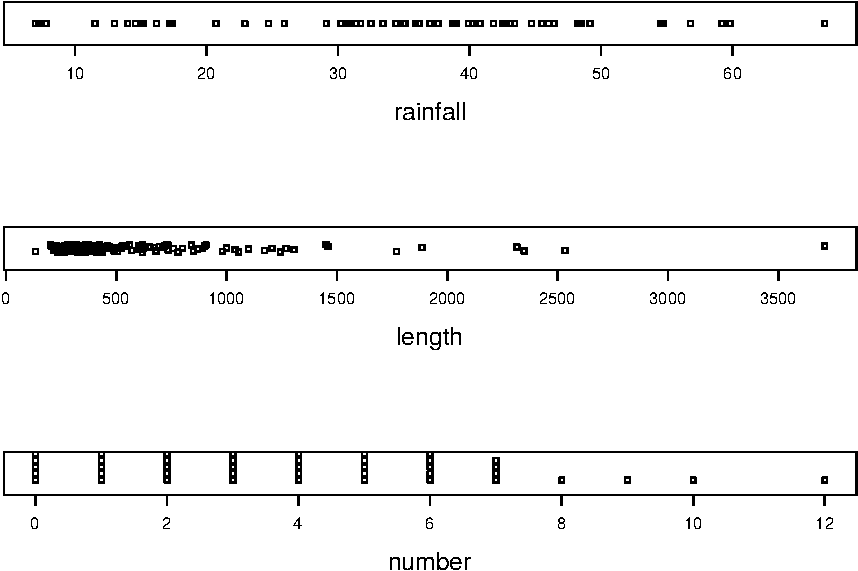
\includegraphics{_main_files/figure-latex/stripcharts-1.pdf}
\caption{\label{fig:stripcharts}\small Three stripcharts of three data sets. The
first graph uses the \texttt{overplot} method, the second the
\texttt{jitter} method, and the third the \texttt{stack} method.}
\end{figure}





The \texttt{DOTplot} \index{DOTplot@\texttt{DOTplot}} function in the
\texttt{UsingR} \index{R packages!UsingR@\texttt{UsingR}} package
\autocite{UsingR} is another alternative.

\subsubsection{\texorpdfstring{Histogram
\index{Histogram}}{Histogram }}\label{histogram}

These are typically used for continuous data. A histogram is constructed
by first deciding on a set of classes, or bins, which partition the real
line into a set of boxes into which the data values fall. Then vertical
bars are drawn over the bins with height proportional to the number of
observations that fell into the bin.

These are one of the most common summary displays, and they are often
misidentified as ``Bar Graphs'' (see below.) The scale on the \(y\) axis
can be frequency, percentage, or density (relative frequency). The term
histogram was coined by Karl Pearson in 1891, see \autocite{Miller}.

\bigskip

\BeginKnitrBlock{example}[Annual Precipitation in US Cities]
\protect\hypertarget{ex:annual}{}{\label{ex:annual} \iffalse (Annual
Precipitation in US Cities) \fi }We are going to take another look at
the \texttt{precip} \index{Data sets!precip@\texttt{precip}} data that
we investigated earlier. The strip chart in Figure \ref{fig:stripcharts}
suggested a loosely balanced distribution; let us now look to see what a
histogram says.
\EndKnitrBlock{example}

There are many ways to plot histograms in R, and one of the easiest is
with the \texttt{hist} \index{hist@\texttt{hist}} function. The
following code produces the plots in Figure \ref{fig-histograms}.

\begin{Shaded}
\begin{Highlighting}[]
\KeywordTok{hist}\NormalTok{(precip, }\DataTypeTok{main =} \StringTok{""}\NormalTok{)}
\KeywordTok{hist}\NormalTok{(precip, }\DataTypeTok{freq =} \OtherTok{FALSE}\NormalTok{, }\DataTypeTok{main =} \StringTok{""}\NormalTok{)}
\end{Highlighting}
\end{Shaded}

Notice the argument \(\mathtt{main = ""}\) which suppresses the main
title from being displayed -- it would have said ``Histogram of
\texttt{precip}'' otherwise. The plot on the left is a frequency
histogram (the default), and the plot on the right is a relative
frequency histogram (\texttt{freq\ =\ FALSE}).

\begin{figure}[htbp]
\centering
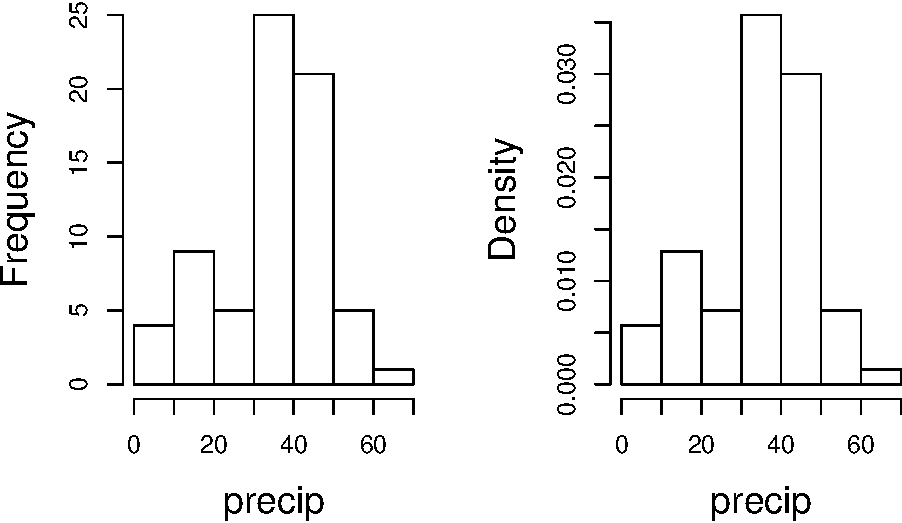
\includegraphics{_main_files/figure-latex/histograms-1.pdf}
\caption{\label{fig:histograms}\small (Relative) frequency histograms of the
\texttt{precip} data.}
\end{figure}




Please mind the biggest weakness of histograms: the graph obtained
strongly depends on the bins chosen. Choose another set of bins, and you
will get a different histogram. Moreover, there are not any definitive
criteria by which bins should be defined; the best choice for a given
data set is the one which illuminates the data set's underlying
structure (if any). Luckily for us there are algorithms to automatically
choose bins that are likely to display well, and more often than not the
default bins do a good job. This is not always the case, however, and a
responsible statistician will investigate many bin choices to test the
stability of the display.

Recall that the strip chart in Figure \ref{fig:stripcharts} suggested a
relatively balanced shape to the \texttt{precip} data distribution.
Watch what happens when we change the bins slightly (with the
\texttt{breaks} argument to \texttt{hist}). See Figure
\ref{fig:histograms-bins} which was produced by the following code.

\begin{Shaded}
\begin{Highlighting}[]
\KeywordTok{hist}\NormalTok{(precip, }\DataTypeTok{breaks =} \DecValTok{10}\NormalTok{)}
\KeywordTok{hist}\NormalTok{(precip, }\DataTypeTok{breaks =} \DecValTok{25}\NormalTok{)}
\KeywordTok{hist}\NormalTok{(precip, }\DataTypeTok{breaks =} \DecValTok{50}\NormalTok{)}
\end{Highlighting}
\end{Shaded}

\begin{figure}[htbp]
\centering
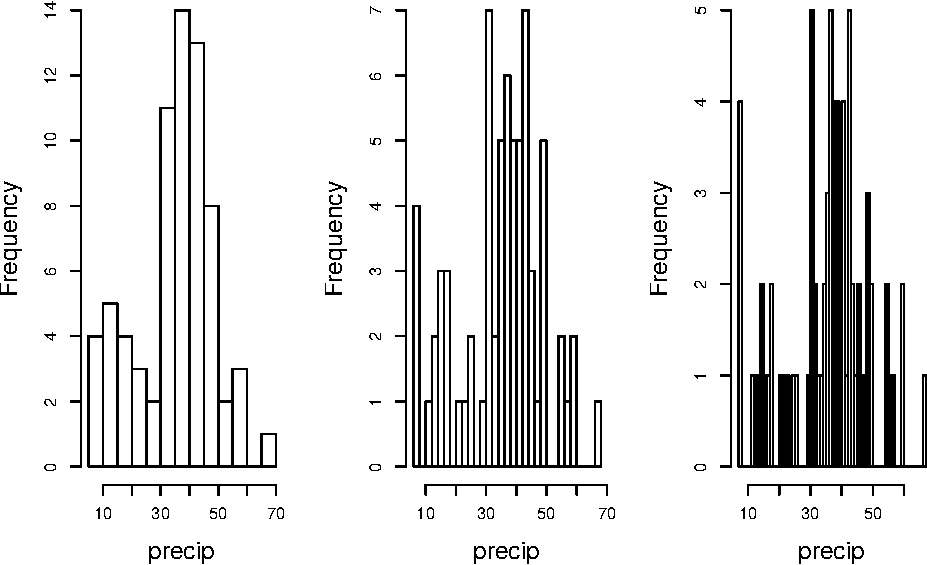
\includegraphics{_main_files/figure-latex/histograms-bins-1.pdf}
\caption{\label{fig:histograms-bins}\small More histograms of the \texttt{precip}
data.}
\end{figure}




The leftmost graph (with \texttt{breaks\ =\ 10}) shows that the
distribution is not balanced at all. There are two humps: a big one in
the middle and a smaller one to the left. Graphs like this often
indicate some underlying group structure to the data; we could now
investigate whether the cities for which rainfall was measured were
similar in some way, with respect to geographic region, for example.

The rightmost graph in Figure \ref{fig:histograms-bins} shows what
happens when the number of bins is too large: the histogram is too
grainy and hides the rounded appearance of the earlier histograms. If we
were to continue increasing the number of bins we would eventually get
all observed bins to have exactly one element, which is nothing more
than a glorified strip chart.

\subsubsection{Stem-and-leaf displays (more to be said in Section
\ref{sec-exploratory-data-analysis})}\label{stem-and-leaf-displays-more-to-be-said-in-section-refsec-exploratory-data-analysis}

Stem-and-leaf displays (also known as stemplots) have two basic parts:
\emph{stems} and \emph{leaves}. The final digit of the data values is
taken to be a \emph{leaf}, and the leading digit(s) is (are) taken to be
\emph{stems}. We draw a vertical line, and to the left of the line we
list the stems. To the right of the line, we list the leaves beside
their corresponding stem. There will typically be several leaves for
each stem, in which case the leaves accumulate to the right. It is
sometimes necessary to round the data values, especially for larger data
sets.

\bigskip

\BeginKnitrBlock{example}[Driver Deaths in the United Kingdom]
\protect\hypertarget{ex:ukdriverdeaths-first}{}{\label{ex:ukdriverdeaths-first}
\iffalse (Driver Deaths in the United Kingdom)
\fi }\texttt{UKDriverDeaths} \index{Data
sets!UKDriverDeaths@\texttt{UKDriverDeaths}} is a time series that
contains the total car drivers killed or seriously injured in Great
Britain monthly from Jan 1969 to Dec 1984. See \texttt{?UKDriverDeaths}.
Compulsory seat belt use was introduced on January 31, 1983. We
construct a stem and leaf diagram in R with the \texttt{stem.leaf}
\index{stem.leaf@\texttt{stem.leaf}} function from the \texttt{aplpack}
\index{R packages@\textsf{R}
packages!aplpack@\texttt{aplpack}} package \autocite{aplpack}.
\EndKnitrBlock{example}

\begin{Shaded}
\begin{Highlighting}[]
\KeywordTok{stem.leaf}\NormalTok{(UKDriverDeaths, }\DataTypeTok{depth =} \OtherTok{FALSE}\NormalTok{)}
\end{Highlighting}
\end{Shaded}

\begin{verbatim}
1 | 2: represents 120
 leaf unit: 10
            n: 192
   10 | 57
   11 | 136678
   12 | 123889
   13 | 0255666888899
   14 | 00001222344444555556667788889
   15 | 0000111112222223444455555566677779
   16 | 01222333444445555555678888889
   17 | 11233344566667799
   18 | 00011235568
   19 | 01234455667799
   20 | 0000113557788899
   21 | 145599
   22 | 013467
   23 | 9
   24 | 7
HI: 2654
\end{verbatim}

The display shows a more or less balanced mound-shaped distribution,
with one or maybe two humps, a big one and a smaller one just to its
right. Note that the data have been rounded to the tens place so that
each datum gets only one leaf to the right of the dividing line.

Notice that the \texttt{depth}s \index{depths} have been suppressed. To
learn more about this option and many others, see Section
\ref{sec-exploratory-data-analysis}. Unlike a histogram, the original
data values may be recovered from the stem-and-leaf display -- modulo
the rounding -- that is, starting from the top and working down we can
read off the data values 1050, 1070, 1110, 1130, and so forth.

\subsubsection{Index plots}\label{index-plots}

Done with the \texttt{plot} \index{plot@\texttt{plot}} function. These
are good for plotting data which are ordered, for example, when the data
are measured over time. That is, the first observation was measured at
time 1, the second at time 2, \emph{etc}. It is a two dimensional plot,
in which the index (or time) is the \(x\) variable and the measured
value is the \(y\) variable. There are several plotting methods for
index plots, and we mention two of them:

\begin{itemize}
\tightlist
\item
  \texttt{spikes}: draws a vertical line from the \(x\)-axis to the
  observation height.
\item
  \texttt{points}: plots a simple point at the observation height.
\end{itemize}

\bigskip

\BeginKnitrBlock{example}[Level of Lake Huron 1875-1972]
\protect\hypertarget{ex:unnamed-chunk-32}{}{\label{ex:unnamed-chunk-32}
\iffalse (Level of Lake Huron 1875-1972) \fi }Brockwell and Davis
\autocite{Brockwell1991} give the annual measurements of the level (in
feet) of Lake Huron from 1875--1972. The data are stored in the time
series \texttt{LakeHuron}. \index{Data
sets!LakeHuron@\texttt{LakeHuron}} See \texttt{?LakeHuron}. Figure
\ref{fig-indpl-lakehuron} was produced with the following code:
\EndKnitrBlock{example}

\begin{Shaded}
\begin{Highlighting}[]
\KeywordTok{plot}\NormalTok{(LakeHuron)}
\KeywordTok{plot}\NormalTok{(LakeHuron, }\DataTypeTok{type =} \StringTok{"p"}\NormalTok{)}
\KeywordTok{plot}\NormalTok{(LakeHuron, }\DataTypeTok{type =} \StringTok{"h"}\NormalTok{)}
\end{Highlighting}
\end{Shaded}

The plots show an overall decreasing trend to the observations, and
there appears to be some seasonal variation that increases over time.

\begin{figure}[htbp]
\centering
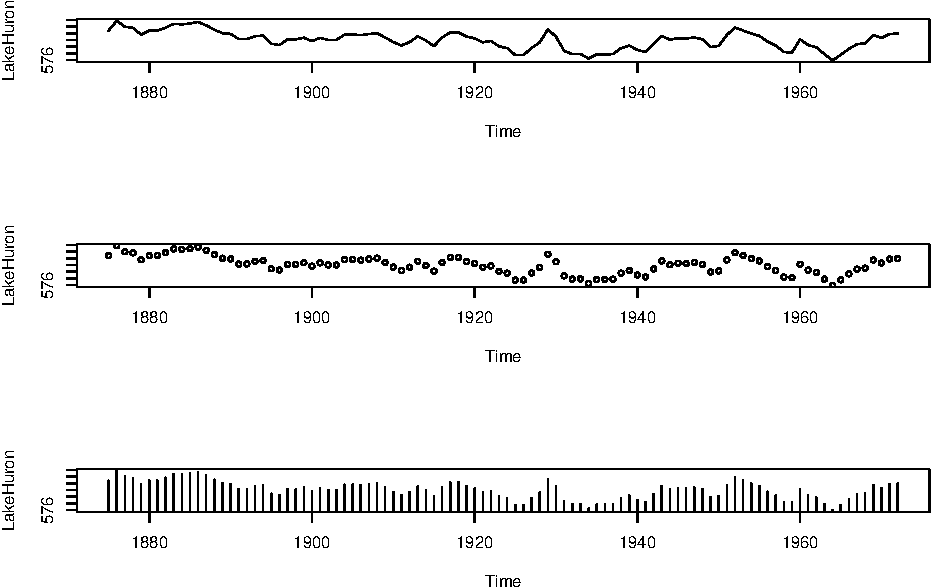
\includegraphics{_main_files/figure-latex/unnamed-chunk-34-1.pdf}
\caption{\label{fig:unnamed-chunk-34}\small Index plots of the \texttt{LakeHuron} data.}
\end{figure}



\subsubsection{Density estimates}\label{density-estimates}

The default method uses a Gaussian kernel density estimate.

\begin{Shaded}
\begin{Highlighting}[]
\CommentTok{# The Old Faithful geyser data}
\NormalTok{d <-}\StringTok{ }\KeywordTok{density}\NormalTok{(faithful$eruptions, }\DataTypeTok{bw =} \StringTok{"sj"}\NormalTok{)}
\NormalTok{d}
\KeywordTok{plot}\NormalTok{(d)}
\KeywordTok{hist}\NormalTok{(precip, }\DataTypeTok{freq =} \OtherTok{FALSE}\NormalTok{)}
\KeywordTok{lines}\NormalTok{(}\KeywordTok{density}\NormalTok{(precip))}
\end{Highlighting}
\end{Shaded}

\subsection{Qualitative Data, Categorical Data, and
Factors}\label{sub-qualitative-data}

Qualitative data are simply any type of data that are not numerical, or
do not represent numerical quantities. Examples of qualitative variables
include a subject's name, gender, race/ethnicity, political party,
socioeconomic status, class rank, driver's license number, and social
security number (SSN).

Please bear in mind that some data \emph{look} to be quantitative but
are \emph{not}, because they do not represent numerical quantities and
do not obey mathematical rules. For example, a person's shoe size is
typically written with numbers: 8, or 9, or 12, or \(12\,\frac{1}{2}\).
Shoe size is not quantitative, however, because if we take a size 8 and
combine with a size 9 we do not get a size 17.

Some qualitative data serve merely to \emph{identify} the observation
(such a subject's name, driver's license number, or SSN). This type of
data does not usually play much of a role in statistics. But other
qualitative variables serve to \emph{subdivide} the data set into
categories; we call these \emph{factors}. In the above examples, gender,
race, political party, and socioeconomic status would be considered
factors (shoe size would be another one). The possible values of a
factor are called its \emph{levels}. For instance, the factor of gender
would have two levels, namely, male and female. Socioeconomic status
typically has three levels: high, middle, and low.

Factors may be of two types: \emph{nominal} \index{nominal data} and
\emph{ordinal}. \index{ordinal data} Nominal factors have levels that
correspond to names of the categories, with no implied ordering.
Examples of nominal factors would be hair color, gender, race, or
political party. There is no natural ordering to ``Democrat'' and
``Republican''; the categories are just names associated with different
groups of people.

In contrast, ordinal factors have some sort of ordered structure to the
underlying factor levels. For instance, socioeconomic status would be an
ordinal categorical variable because the levels correspond to ranks
associated with income, education, and occupation. Another example of
ordinal categorical data would be class rank.

Factors have special status in R. They are represented internally by
numbers, but even when they are written numerically their values do not
convey any numeric meaning or obey any mathematical rules (that is,
Stage III cancer is not Stage I cancer + Stage II cancer).

\bigskip

\BeginKnitrBlock{example}
\protect\hypertarget{ex:unnamed-chunk-36}{}{\label{ex:unnamed-chunk-36}}The
\texttt{state.abb} \index{Data sets!state.abb@\texttt{state.abb}} vector
gives the two letter postal abbreviations for all 50 states.
\EndKnitrBlock{example}

\begin{Shaded}
\begin{Highlighting}[]
\KeywordTok{str}\NormalTok{(state.abb)}
\end{Highlighting}
\end{Shaded}

\begin{verbatim}
 chr [1:50] "AL" "AK" "AZ" "AR" "CA" "CO" ...
\end{verbatim}

These would be ID data. The \texttt{state.name} \index{Data
sets!state.name@\texttt{state.name}} vector lists all of the complete
names and those data would also be ID.

\bigskip

\BeginKnitrBlock{example}[U.S. State Facts and Features]
\protect\hypertarget{ex:unnamed-chunk-38}{}{\label{ex:unnamed-chunk-38}
\iffalse (U.S. State Facts and Features) \fi }The U.S. Department of
Commerce of the U.S. Census Bureau releases all sorts of information in
the \emph{Statistical Abstract of the United States}, and the
\texttt{state.region} \index{Data
sets!state.region@\texttt{state.region}} data lists each of the 50
states and the region to which it belongs, be it Northeast, South, North
Central, or West. See \texttt{?state.region}.
\EndKnitrBlock{example}

\begin{Shaded}
\begin{Highlighting}[]
\KeywordTok{str}\NormalTok{(state.region)}
\end{Highlighting}
\end{Shaded}

\begin{verbatim}
 Factor w/ 4 levels "Northeast","South",..: 2 4 4 2 4 4 1 2 2 2 ...
\end{verbatim}

\begin{Shaded}
\begin{Highlighting}[]
\NormalTok{state.region[}\DecValTok{1}\NormalTok{:}\DecValTok{5}\NormalTok{]}
\end{Highlighting}
\end{Shaded}

\begin{verbatim}
[1] South West  West  South West 
Levels: Northeast South North Central West
\end{verbatim}

The \texttt{str} \index{str@\texttt{str}} output shows that
\texttt{state.region} is already stored internally as a factor and it
lists a couple of the factor levels. To see all of the levels we printed
the first five entries of the vector in the second line.

\subsection{Displaying Qualitative
Data}\label{sub-displaying-qualitative-data}

\subsubsection{Tables}\label{par-tables}

One of the best ways to summarize qualitative data is with a table of
the data values. We may count frequencies with the \texttt{table}
function or list proportions with the \texttt{prop.table}
\index{prop.table@\texttt{prop.table}} function (whose input is a
frequency table). In the R Commander you can do it with
\texttt{Statistics} \(\triangleright\)
\texttt{Frequency\ Distribution...} Alternatively, to look at tables for
all factors in the \texttt{Active\ data\ set}
\index{Active data set@\texttt{Active data set}} you can do
\texttt{Statistics} \(\triangleright\) \texttt{Summaries}
\(\triangleright\) \texttt{Active\ Dataset}.

\begin{Shaded}
\begin{Highlighting}[]
\NormalTok{Tbl <-}\StringTok{ }\KeywordTok{table}\NormalTok{(state.division)}
\NormalTok{Tbl}
\end{Highlighting}
\end{Shaded}

\begin{verbatim}
state.division
       New England    Middle Atlantic     South Atlantic 
                 6                  3                  8 
East South Central West South Central East North Central 
                 4                  4                  5 
West North Central           Mountain            Pacific 
                 7                  8                  5 
\end{verbatim}

\begin{Shaded}
\begin{Highlighting}[]
\NormalTok{Tbl/}\KeywordTok{sum}\NormalTok{(Tbl)      }\CommentTok{# relative frequencies}
\end{Highlighting}
\end{Shaded}

\begin{verbatim}
state.division
       New England    Middle Atlantic     South Atlantic 
              0.12               0.06               0.16 
East South Central West South Central East North Central 
              0.08               0.08               0.10 
West North Central           Mountain            Pacific 
              0.14               0.16               0.10 
\end{verbatim}

\begin{Shaded}
\begin{Highlighting}[]
\KeywordTok{prop.table}\NormalTok{(Tbl)   }\CommentTok{# same thing}
\end{Highlighting}
\end{Shaded}

\begin{verbatim}
state.division
       New England    Middle Atlantic     South Atlantic 
              0.12               0.06               0.16 
East South Central West South Central East North Central 
              0.08               0.08               0.10 
West North Central           Mountain            Pacific 
              0.14               0.16               0.10 
\end{verbatim}

\subsubsection{Bar Graphs}\label{par-bar-graphs}

A bar graph is the analogue of a histogram for categorical data. A bar
is displayed for each level of a factor, with the heights of the bars
proportional to the frequencies of observations falling in the
respective categories. A disadvantage of bar graphs is that the levels
are ordered alphabetically (by default), which may sometimes obscure
patterns in the display.

\bigskip

\BeginKnitrBlock{example}[U.S. State Facts and Features]
\protect\hypertarget{ex:unnamed-chunk-43}{}{\label{ex:unnamed-chunk-43}
\iffalse (U.S. State Facts and Features) \fi }The \texttt{state.region}
data lists each of the 50 states and the region to which it belongs, be
it Northeast, South, North Central, or West. See \texttt{?state.region}.
It is already stored internally as a factor. We make a bar graph with
the \texttt{barplot} \index{barplot@\texttt{barplot}} function:
\EndKnitrBlock{example}

\begin{Shaded}
\begin{Highlighting}[]
\KeywordTok{barplot}\NormalTok{(}\KeywordTok{table}\NormalTok{(state.region), }\DataTypeTok{cex.names =} \FloatTok{1.20}\NormalTok{)}
\KeywordTok{barplot}\NormalTok{(}\KeywordTok{prop.table}\NormalTok{(}\KeywordTok{table}\NormalTok{(state.region)), }\DataTypeTok{cex.names =} \FloatTok{1.20}\NormalTok{)}
\end{Highlighting}
\end{Shaded}

See Figure \ref{fig:bar-gr-stateregion}. The display on the left is a
frequency bar graph because the \(y\) axis shows counts, while the
display on the left is a relative frequency bar graph. The only
difference between the two is the scale. Looking at the graph we see
that the majority of the fifty states are in the South, followed by
West, North Central, and finally Northeast. Over 30\% of the states are
in the South.

Notice the \texttt{cex.names} \index{cex.names@\texttt{cex.names}}
argument that we used, above. It expands the names on the \(x\) axis by
20\% which makes them easier to read. See \texttt{?par}
\index{par@\texttt{par}} for a detailed list of additional plot
parameters.

\begin{figure}[htbp]
\centering
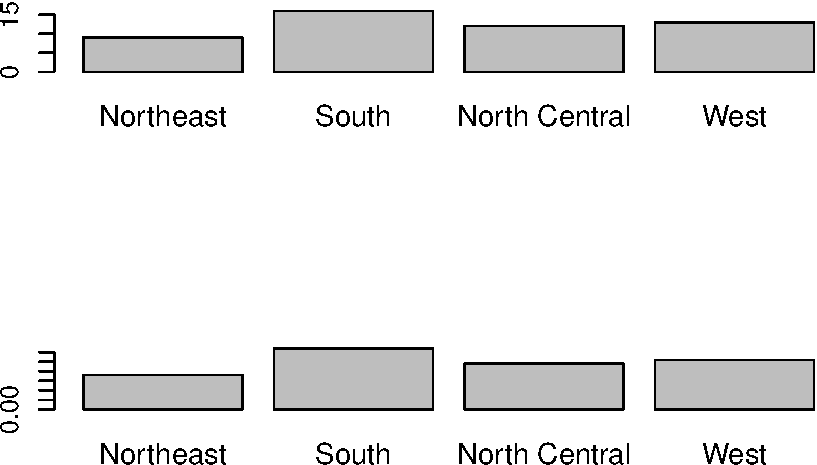
\includegraphics{_main_files/figure-latex/bar-gr-stateregion-1.pdf}
\caption{\label{fig:bar-gr-stateregion}\small The top graph is a frequency barplot made
with \texttt{table} and the bottom is a relative frequency barplot made
with \texttt{prop.table}.}
\end{figure}





\subsubsection{Pareto Diagrams}\label{par-pareto-diagrams}

A pareto diagram is a lot like a bar graph except the bars are
rearranged such that they decrease in height going from left to right.
The rearrangement is handy because it can visually reveal structure (if
any) in how fast the bars decrease -- this is much more difficult when
the bars are jumbled.

\bigskip

\BeginKnitrBlock{example}[U.S. State Facts and Features]
\protect\hypertarget{ex:unnamed-chunk-45}{}{\label{ex:unnamed-chunk-45}
\iffalse (U.S. State Facts and Features) \fi }The
\texttt{state.division} \index{Data
sets!state.division@\texttt{state.division}} data record the division
(New England, Middle Atlantic, South Atlantic, East South Central, West
South Central, East North Central, West North Central, Mountain, and
Pacific) of the fifty states. We can make a pareto diagram with either
the \texttt{RcmdrPlugin.IPSUR} \index{R
packages@\textsf{R}
packages!RcmdrPlugin.IPSUR@\texttt{RcmdrPlugin.IPSUR}} package
\autocite{RcmdrPlugin.IPSUR} or with the \texttt{pareto.chart}
\index{pareto.chart@\texttt{pareto.chart}} function from the
\texttt{qcc} \index{R packages@\textsf{R}
packages!qcc@\texttt{qcc}} package \autocite{qcc}. See Figure
\ref{fig:pareto-chart}. The code follows.
\EndKnitrBlock{example}

\begin{Shaded}
\begin{Highlighting}[]
\KeywordTok{pareto.chart}\NormalTok{(}\KeywordTok{table}\NormalTok{(state.division), }\DataTypeTok{ylab=}\StringTok{"Frequency"}\NormalTok{, }\DataTypeTok{cex.lab =} \NormalTok{cexlab)}
\end{Highlighting}
\end{Shaded}

\begin{figure}[htbp]
\centering
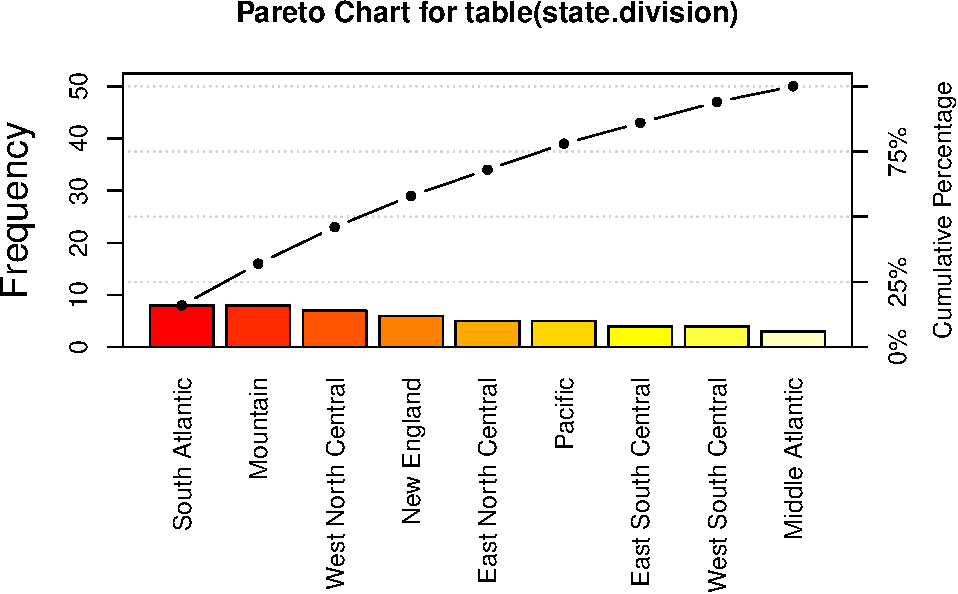
\includegraphics{_main_files/figure-latex/pareto-chart-1.pdf}
\caption{\label{fig:pareto-chart}\small Pareto chart of the \texttt{state.division}
data.}
\end{figure}

\begin{verbatim}
                    
Pareto chart analysis for table(state.division)
                     Frequency Cum.Freq. Percentage
  South Atlantic             8         8         16
  Mountain                   8        16         16
  West North Central         7        23         14
  New England                6        29         12
  East North Central         5        34         10
  Pacific                    5        39         10
  East South Central         4        43          8
  West South Central         4        47          8
  Middle Atlantic            3        50          6
                    
Pareto chart analysis for table(state.division)
                     Cum.Percent.
  South Atlantic               16
  Mountain                     32
  West North Central           46
  New England                  58
  East North Central           68
  Pacific                      78
  East South Central           86
  West South Central           94
  Middle Atlantic             100
\end{verbatim}




\subsubsection{Dot Charts}\label{par-dotcharts}

These are a lot like a bar graph that has been turned on its side with
the bars replaced by dots on horizontal lines. They do not convey any
more (or less) information than the associated bar graph, but the
strength lies in the economy of the display. Dot charts are so compact
that it is easy to graph very complicated multi-variable interactions
together in one graph. See Section \ref{sec-comparing-data-sets}. We
will give an example here using the same data as above for comparison.
The graph was produced by the following code.

\begin{Shaded}
\begin{Highlighting}[]
\NormalTok{x <-}\StringTok{ }\KeywordTok{table}\NormalTok{(state.region)}
\KeywordTok{dotchart}\NormalTok{(}\KeywordTok{as.vector}\NormalTok{(x), }\DataTypeTok{labels =} \KeywordTok{names}\NormalTok{(x), }\DataTypeTok{cex.lab =} \NormalTok{cexlab)}
\end{Highlighting}
\end{Shaded}

\begin{figure}[htbp]
\centering
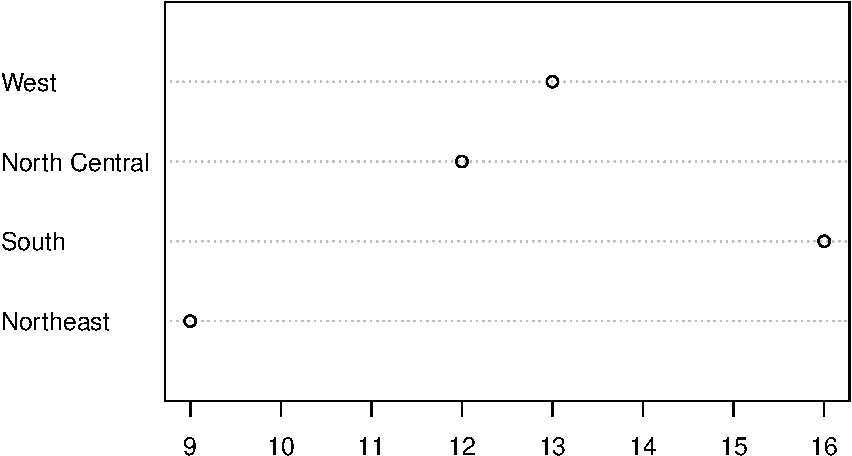
\includegraphics{_main_files/figure-latex/dotchart-1.pdf}
\caption{\label{fig:dotchart}\small Dot chart of the \texttt{state.region} data.}
\end{figure}



See Figure \ref{fig:dotchart}. Compare it to Figure
\ref{fig:bar-gr-stateregion}.

\subsubsection{Pie Graphs}\label{par-pie-graphs}

These can be done with R and the R Commander, but they fallen out of
favor in recent years because researchers have determined that while the
human eye is good at judging linear measures, it is notoriously bad at
judging relative areas (such as those displayed by a pie graph). Pie
charts are consequently a very bad way of displaying information unless
the number of categories is two or three. A bar chart or dot chart is a
preferable way of displaying qualitative data. See \texttt{?pie}
\index{pie@\texttt{pie}} for more information.

We are not going to do any examples of a pie graph and discourage their
use elsewhere.

\subsection{Logical Data}\label{sub-logical-data}

There is another type of information recognized by R which does not fall
into the above categories. The value is either \texttt{TRUE} or
\texttt{FALSE} (note that equivalently you can use \texttt{1\ =\ TRUE},
\texttt{0\ =\ FALSE}). Here is an example of a logical vector:

\begin{Shaded}
\begin{Highlighting}[]
\NormalTok{x <-}\StringTok{ }\DecValTok{5}\NormalTok{:}\DecValTok{9}
\NormalTok{y <-}\StringTok{ }\NormalTok{(x <}\StringTok{ }\FloatTok{7.3}\NormalTok{)}
\NormalTok{y}
\end{Highlighting}
\end{Shaded}

\begin{verbatim}
[1]  TRUE  TRUE  TRUE FALSE FALSE
\end{verbatim}

Many functions in R have options that the user may or may not want to
activate in the function call. For example, the \texttt{stem.leaf}
function has the \texttt{depths} argument which is \texttt{TRUE} by
default. We saw in Section {[}{[}\#sub-Quantitative-Data{]}{]} how to
turn the option off, simply enter
\texttt{stem.leaf(x,\ depths\ =\ FALSE)} and they will not be shown on
the display.

We can swap \texttt{TRUE} with \texttt{FALSE} with the exclamation point
\texttt{!}.

\begin{Shaded}
\begin{Highlighting}[]
\NormalTok{!y}
\end{Highlighting}
\end{Shaded}

\begin{verbatim}
[1] FALSE FALSE FALSE  TRUE  TRUE
\end{verbatim}

\subsection{Missing Data}\label{sub-missing-data}

Missing data are a persistent and prevalent problem in many statistical
analyses, especially those associated with the social sciences. R
reserves the special symbol \texttt{NA} to representing missing data.

Ordinary arithmetic with \texttt{NA} values give \texttt{NA}'s
(addition, subtraction, \emph{etc}.) and applying a function to a vector
that has an \texttt{NA} in it will usually give an \texttt{NA}.

\begin{Shaded}
\begin{Highlighting}[]
\NormalTok{x <-}\StringTok{ }\KeywordTok{c}\NormalTok{(}\DecValTok{3}\NormalTok{, }\DecValTok{7}\NormalTok{, }\OtherTok{NA}\NormalTok{, }\DecValTok{4}\NormalTok{, }\DecValTok{7}\NormalTok{)}
\NormalTok{y <-}\StringTok{ }\KeywordTok{c}\NormalTok{(}\DecValTok{5}\NormalTok{, }\OtherTok{NA}\NormalTok{, }\DecValTok{1}\NormalTok{, }\DecValTok{2}\NormalTok{, }\DecValTok{2}\NormalTok{)}
\NormalTok{x +}\StringTok{ }\NormalTok{y}
\end{Highlighting}
\end{Shaded}

\begin{verbatim}
[1]  8 NA NA  6  9
\end{verbatim}

Some functions have a \texttt{na.rm} argument which when \texttt{TRUE}
will ignore missing data as if they were not there (such as
\texttt{mean}, \texttt{var}, \texttt{sd}, \texttt{IQR}, \texttt{mad},
\ldots{}).

\begin{Shaded}
\begin{Highlighting}[]
\KeywordTok{sum}\NormalTok{(x)}
\end{Highlighting}
\end{Shaded}

\begin{verbatim}
[1] NA
\end{verbatim}

\begin{Shaded}
\begin{Highlighting}[]
\KeywordTok{sum}\NormalTok{(x, }\DataTypeTok{na.rm =} \OtherTok{TRUE}\NormalTok{)}
\end{Highlighting}
\end{Shaded}

\begin{verbatim}
[1] 21
\end{verbatim}

Other functions do not have a \texttt{na.rm} argument and will return
\texttt{NA} or an error if the argument has \texttt{NA}s. In those cases
we can find the locations of any \texttt{NA}s with the \texttt{is.na}
function and remove those cases with the \texttt{{[}{]}} operator.

\begin{Shaded}
\begin{Highlighting}[]
\KeywordTok{is.na}\NormalTok{(x)}
\end{Highlighting}
\end{Shaded}

\begin{verbatim}
[1] FALSE FALSE  TRUE FALSE FALSE
\end{verbatim}

\begin{Shaded}
\begin{Highlighting}[]
\NormalTok{z <-}\StringTok{ }\NormalTok{x[!}\KeywordTok{is.na}\NormalTok{(x)]}
\KeywordTok{sum}\NormalTok{(z)}
\end{Highlighting}
\end{Shaded}

\begin{verbatim}
[1] 21
\end{verbatim}

The analogue of \texttt{is.na} for rectangular data sets (or data
frames) is the \texttt{complete.cases} function. See Appendix
\ref{sec-editing-data-sets}.

\subsection{Other Data Types}\label{sub-other-data-types}

\section{Features of Data Distributions}\label{sec-features-of-data}

Given that the data have been appropriately displayed, the next step is
to try to identify salient features represented in the graph. The
acronym to remember is \emph{C}-enter, \emph{U}-nusual features,
\emph{S}-pread, and \emph{S}-hape. (CUSS).

\subsection{Center}\label{sub-center}

One of the most basic features of a data set is its center. Loosely
speaking, the center of a data set is associated with a number that
represents a middle or general tendency of the data. Of course, there
are usually several values that would serve as a center, and our later
tasks will be focused on choosing an appropriate one for the data at
hand. Judging from the histogram that we saw in Figure
\ref{fig:histograms-bins}, a measure of center would be about 35.

\subsection{Spread}\label{sub-spread}

The spread of a data set is associated with its variability; data sets
with a large spread tend to cover a large interval of values, while data
sets with small spread tend to cluster tightly around a central value.

\subsection{Shape}\label{sub-shape}

When we speak of the \emph{shape} of a data set, we are usually
referring to the shape exhibited by an associated graphical display,
such as a histogram. The shape can tell us a lot about any underlying
structure to the data, and can help us decide which statistical
procedure we should use to analyze them.

\subsubsection{Symmetry and Skewness}\label{symmetry-and-skewness}

A distribution is said to be \emph{right-skewed} (or \emph{positively
skewed}) if the right tail seems to be stretched from the center. A
\emph{left-skewed} (or \emph{negatively skewed}) distribution is
stretched to the left side. A symmetric distribution has a graph that is
balanced about its center, in the sense that half of the graph may be
reflected about a central line of symmetry to match the other half.

We have already encountered skewed distributions: both the discoveries
data in Figure \ref{fig:stripcharts} and the \texttt{precip} data in
Figure \ref{fig:histograms-bins} appear right-skewed. The
\texttt{UKDriverDeaths} data in Example \ref{ex:ukdriverdeaths-first} is
relatively symmetric (but note the one extreme value 2654 identified at
the bottom of the stem-and-leaf display).

\subsubsection{Kurtosis}\label{kurtosis}

Another component to the shape of a distribution is how ``peaked'' it
is. Some distributions tend to have a flat shape with thin tails. These
are called \emph{platykurtic}, and an example of a platykurtic
distribution is the uniform distribution; see Section
\ref{sec-the-continuous-uniform}. On the other end of the spectrum are
distributions with a steep peak, or spike, accompanied by heavy tails;
these are called \emph{leptokurtic}. Examples of leptokurtic
distributions are the Laplace distribution and the logistic
distribution. See Section \ref{sec-other-continuous-distributions}. In
between are distributions (called \emph{mesokurtic}) with a rounded peak
and moderately sized tails. The standard example of a mesokurtic
distribution is the famous bell-shaped curve, also known as the
Gaussian, or normal, distribution, and the binomial distribution can be
mesokurtic for specific choices of \(p\). See Sections
\ref{sec-binom-dist} and \ref{sec-the-normal-distribution}.

\subsection{Clusters and Gaps}\label{sub-clusters-and-gaps}

Clusters or gaps are sometimes observed in quantitative data
distributions. They indicate clumping of the data about distinct values,
and gaps may exist between clusters. Clusters often suggest an
underlying grouping to the data. For example, take a look at the
\texttt{faithful} data which contains the duration of \texttt{eruptions}
and the \texttt{waiting} time between eruptions of the Old Faithful
geyser in Yellowstone National Park. Do not be frightened by the
complicated information at the left of the display for now; we will
learn how to interpret it in Section
\ref{sec-exploratory-data-analysis}.

\begin{Shaded}
\begin{Highlighting}[]
\KeywordTok{with}\NormalTok{(faithful, }\KeywordTok{stem.leaf}\NormalTok{(eruptions))}
\end{Highlighting}
\end{Shaded}

\begin{verbatim}
1 | 2: represents 1.2
 leaf unit: 0.1
            n: 272
   12     s | 667777777777
   51    1. | 888888888888888888888888888899999999999
   71    2* | 00000000000011111111
   87     t | 2222222222333333
   92     f | 44444
   94     s | 66
   97    2. | 889
   98    3* | 0
  102     t | 3333
  108     f | 445555
  118     s | 6666677777
  (16)   3. | 8888888889999999
  138    4* | 0000000000000000111111111111111
  107     t | 22222222222233333333333333333
   78     f | 44444444444445555555555555555555555
   43     s | 6666666666677777777777
   21    4. | 88888888888899999
    4    5* | 0001
\end{verbatim}

There are definitely two clusters of data here; an upper cluster and a
lower cluster.

\subsection{Extreme Observations and other Unusual
Features}\label{sub-extreme-observations}

Extreme observations fall far from the rest of the data. Such
observations are troublesome to many statistical procedures; they cause
exaggerated estimates and instability. It is important to identify
extreme observations and examine the source of the data more closely.
There are many possible reasons underlying an extreme observation:

\begin{itemize}
\tightlist
\item
  \emph{Maybe the value is a typographical error.} Especially with large
  data sets becoming more prevalent, many of which being recorded by
  hand, mistakes are a common problem. After closer scrutiny, these can
  often be fixed.
\item
  \emph{Maybe the observation was not meant for the study}, because it
  does not belong to the population of interest. For example, in medical
  research some subjects may have relevant complications in their
  genealogical history that would rule out their participation in the
  experiment. Or when a manufacturing company investigates the
  properties of one of its devices, perhaps a particular product is
  malfunctioning and is not representative of the majority of the items.
\item
  \emph{Maybe it indicates a deeper trend or phenomenon.} Many of the
  most influential scientific discoveries were made when the
  investigator noticed an unexpected result, a value that was not
  predicted by the classical theory. Albert Einstein, Louis Pasteur, and
  others built their careers on exactly this circumstance.
\end{itemize}

\section{Descriptive Statistics}\label{sec-descriptive-statistics}

One of my favorite professors would repeatedly harp, ``You cannot do
statistics without data.''

\textbf{What do I want them to know?}

\begin{itemize}
\tightlist
\item
  The fundamental data types we encounter most often, how to classify
  given data into a likely type, and that sometimes the distinction is
  blurry.
\end{itemize}

\subsection{Frequencies and Relative
Frequencies}\label{sub-frequencies-and-relative}

These are used for categorical data. The idea is that there are a number
of different categories, and we would like to get some idea about how
the categories are represented in the population.

\subsection{Measures of Center}\label{sub-measures-of-center}

The \emph{sample mean} is denoted \(\overline{x}\) (read ``\(x\)-bar'')
and is simply the arithmetic average of the observations:

\begin{equation} 
\overline{x}=\frac{x_{1}+x_{2}+\cdots+x_{n}}{n}=\frac{1}{n}\sum_{i=1}^{n}x_{i}.
\end{equation}

\begin{itemize}
\tightlist
\item
  Good: natural, easy to compute, has nice mathematical properties
\item
  Bad: sensitive to extreme values
\end{itemize}

It is appropriate for use with data sets that are not highly skewed
without extreme observations.

The \emph{sample median} is another popular measure of center and is
denoted \(\tilde{x}\). To calculate its value, first sort the data into
an increasing sequence of numbers. If the data set has an odd number of
observations then \(\tilde{x}\) is the value of the middle observation,
which lies in position \((n+1)/2\); otherwise, there are two middle
observations and \(\tilde{x}\) is the average of those middle values.

\begin{itemize}
\tightlist
\item
  Good: resistant to extreme values, easy to describe
\item
  Bad: not as mathematically tractable, need to sort the data to
  calculate
\end{itemize}

One desirable property of the sample median is that it is
\emph{resistant} to extreme observations, in the sense that the value of
\(\tilde{x}\) depends only on those data values in the middle, and is
quite unaffected by the actual values of the outer observations in the
ordered list. The same cannot be said for the sample mean. Any
significant changes in the magnitude of an observation \(x_{k}\) results
in a corresponding change in the value of the mean. Consequently, the
sample mean is said to be \emph{sensitive} to extreme observations.

The \emph{trimmed mean} is a measure designed to address the sensitivity
of the sample mean to extreme observations. The idea is to ``trim'' a
fraction (less than 1/2) of the observations off each end of the ordered
list, and then calculate the sample mean of what remains. We will denote
it by \(\overline{x}_{t=0.05}\).

\begin{itemize}
\tightlist
\item
  Good: resistant to extreme values, shares nice statistical properties
\item
  Bad: need to sort the data
\end{itemize}

\subsubsection{How to do it with R}\label{how-to-do-it-with-r}

\begin{itemize}
\tightlist
\item
  You can calculate frequencies or relative frequencies with the
  \texttt{table} function, and relative frequencies with
  \texttt{prop.table(table())}.
\item
  You can calculate the sample mean of a data vector \texttt{x} with the
  command \texttt{mean(x)}.
\item
  You can calculate the sample median of \texttt{x} with the command
  \texttt{median(x)}.
\item
  You can calculate the trimmed mean with the \texttt{trim} argument;
  \texttt{mean(x,\ trim\ =\ 0.05)}.
\end{itemize}

\subsection{Order Statistics and the Sample
Quantiles}\label{sub-order-statistics}

A common first step in an analysis of a data set is to sort the values.
Given a data set \(x_{1}\), \(x_{2}\), \ldots{}, \(x_{n}\), we may sort
the values to obtain an increasing sequence

\begin{equation} 
x_{(1)}\leq x_{(2)}\leq x_{(3)}\leq\cdots\leq x_{(n)}
\end{equation}

and the resulting values are called the \emph{order statistics}. The
\(k^{\mathrm{th}}\) entry in the list, \(x_{(k)}\), is the
\(k^{\mathrm{th}}\) order statistic, and approximately \(100(k/n)\)\% of
the observations fall below \(x_{(k)}\). The order statistics give an
indication of the shape of the data distribution, in the sense that a
person can look at the order statistics and have an idea about where the
data are concentrated, and where they are sparse.

The \emph{sample quantiles} are related to the order statistics.
Unfortunately, there is not a universally accepted definition of them.
Indeed, R is equipped to calculate quantiles using nine distinct
definitions! We will describe the default method (\texttt{type\ =\ 7}),
but the interested reader can see the details for the other methods with
\texttt{?quantile}.

Suppose the data set has \(n\) observations. Find the sample quantile of
order \(p\) (\(0<p<1\)), denoted \(\tilde{q}_{p}\) , as follows:

\begin{itemize}
\tightlist
\item
  \textbf{First step:} sort the data to obtain the order statistics
  \(x_{(1)}\), \(x_{(2)}\), \ldots{},\(x_{(n)}\).
\item
  \textbf{Second step:} calculate \((n-1)p+1\) and write it in the form
  \(k.d\), where \(k\) is an integer and \(d\) is a decimal.
\item
  \textbf{Third step:} The sample quantile \(\tilde{q}_{p}\) is

  \begin{equation}
    \tilde{q}_{p}=x_{(k)}+d(x_{(k+1)}-x_{(k)}).
     \end{equation}
\end{itemize}

The interpretation of \(\tilde{q}_{p}\) is that approximately \(100p\)
\% of the data fall below the value \(\tilde{q}_{p}\).

Keep in mind that there is not a unique definition of percentiles,
quartiles, \emph{etc}. Open a different book, and you'll find a
different definition. The difference is small and seldom plays a role
except in small data sets with repeated values. In fact, most people do
not even notice in common use.

Clearly, the most popular sample quantile is \(\tilde{q}_{0.50}\), also
known as the sample median, \(\tilde{x}\). The closest runners-up are
the \emph{first quartile} \(\tilde{q}_{0.25}\) and the \emph{third
quartile} \(\tilde{q}_{0.75}\) (the \emph{second quartile} is the
median).

\subsubsection{How to do it with R}\label{how-to-do-it-with-r-1}

\textbf{At the command prompt} We can find the order statistics of a
data set stored in a vector \texttt{x} with the command
\texttt{sort(x)}.

We can calculate the sample quantiles of any order \(p\) where \(0<p<1\)
for a data set stored in a data vector \texttt{x} with the
\texttt{quantile} function, for instance, the command
\texttt{quantile(x,\ probs\ =\ c(0,\ 0.25,\ 0.37))} will return the
smallest observation, the first quartile, \(\tilde{q}_{0.25}\), and the
37th sample quantile, \(\tilde{q}_{0.37}\). For \(\tilde{q}_{p}\) simply
change the values in the \texttt{probs} argument to the value \(p\).

\textbf{With the R Commander} we can find the order statistics of a
variable in the \texttt{Active\ data\ set} by doing \texttt{Data}
\(\triangleright\) \texttt{Manage\ variables\ in\ Active\ data\ set...}
\(\triangleright\) \texttt{Compute\ new\ variable...} In the
\texttt{Expression\ to\ compute} dialog simply type
\texttt{sort(varname)}, where \texttt{varname} is the variable that it
is desired to sort.

In \texttt{Rcmdr}, we can calculate the sample quantiles for a
particular variable with the sequence \texttt{Statistics}
\(\triangleright\) \texttt{Summaries} \(\triangleright\)
\texttt{Numerical\ Summaries...} We can automatically calculate the
quartiles for all variables in the \texttt{Active\ data\ set} with the
sequence \texttt{Statistics} \(\triangleright\) \texttt{Summaries}
\(\triangleright\) \texttt{Active\ Dataset}.

\subsection{Measures of Spread}\label{sub-measures-of-spread}

\subsubsection{Sample Variance and Standard
Deviation}\label{sample-variance-and-standard-deviation}

The \emph{sample variance} is denoted \(s^{2}\) and is calculated with
the formula

\begin{equation}
s^{2}=\frac{1}{n-1}\sum_{i=1}^{n}(x_{i}-\overline{x})^{2}.
\end{equation}

The \emph{sample standard deviation} is \(s=\sqrt{s^{2}}\). Intuitively,
the sample variance is approximately the average squared distance of the
observations from the sample mean. The sample standard deviation is used
to scale the estimate back to the measurement units of the original
data.

\begin{itemize}
\tightlist
\item
  Good: tractable, has nice mathematical/statistical properties
\item
  Bad: sensitive to extreme values
\end{itemize}

We will spend a lot of time with the variance and standard deviation in
the coming chapters. In the meantime, the following two rules give some
meaning to the standard deviation, in that there are bounds on how much
of the data can fall past a certain distance from the mean.

\textbf{Fact:} (Chebychev's Rule). The proportion of observations within
\(k\) standard deviations of the mean is at least \(1-1/k^{2}\),
\emph{i.e.}, at least 75\%, 89\%, and 94\% of the data are within 2, 3,
and 4 standard deviations of the mean, respectively.

Note that Chebychev's Rule does not say anything about when \(k=1\),
because \(1-1/1^{2}=0\), which states that at least 0\% of the
observations are within one standard deviation of the mean (which is not
saying much).

Chebychev's Rule applies to any data distribution, \emph{any} list of
numbers, no matter where it came from or what the histogram looks like.
The price for such generality is that the bounds are not very tight; if
we know more about how the data are shaped then we can say more about
how much of the data can fall a given distance from the mean.

\textbf{Fact:} (Empirical Rule). If data follow a bell-shaped curve,
then approximately 68\%, 95\%, and 99.7\% of the data are within 1, 2,
and 3 standard deviations of the mean, respectively.

\subsubsection{Interquartile Range}\label{interquartile-range}

Just as the sample mean is sensitive to extreme values, so the
associated measure of spread is similarly sensitive to extremes.
Further, the problem is exacerbated by the fact that the extreme
distances are squared. We know that the sample quartiles are resistant
to extremes, and a measure of spread associated with them is the
\emph{interquartile range} (\(IQR\)) defined by
\(IQR=q_{0.75}-q_{0.25}\).

\begin{itemize}
\tightlist
\item
  Good: stable, resistant to outliers, robust to nonnormality, easy to
  explain
\item
  Bad: not as tractable, need to sort the data, only involves the middle
  50\% of the data.
\end{itemize}

\subsubsection{Median Absolute
Deviation}\label{median-absolute-deviation}

A measure even more robust than the \(IQR\) is the \emph{median absolute
deviation} (\(MAD\)). To calculate it we first get the median
\(\widetilde{x}\), next the \emph{absolute deviations}
\(|x_{1}-\tilde{x}|\), \(|x_{2}-\tilde{x}|\), \ldots{},
\(|x_{n}-\tilde{x}|\), and the \(MAD\) is proportional to the median of
those deviations:

\begin{equation}
MAD\propto\mbox{median}(|x_{1}-\tilde{x}|,\ |x_{2}-\tilde{x}|,\ldots,|x_{n}-\tilde{x}|).
\end{equation}

That is, the
\(MAD=c\cdot\mbox{median}(|x_{1}-\tilde{x}|,\ |x_{2}-\tilde{x}|,\ldots,|x_{n}-\tilde{x}|)\),
where \(c\) is a constant chosen so that the \(MAD\) has nice
properties. The value of \(c\) in R is by default \(c=1.4286\). This
value is chosen to ensure that the estimator of \(\sigma\) is correct,
on the average, under suitable sampling assumptions (see Section
\ref{sec-point-estimation}).

\begin{itemize}
\tightlist
\item
  Good: stable, very robust, even more so than the \(IQR\).
\item
  Bad: not tractable, not well known and less easy to explain.
\end{itemize}

\subsubsection{Comparing Apples to
Apples}\label{comparing-apples-to-apples}

We have seen three different measures of spread which, for a given data
set, will give three different answers. Which one should we use? It
depends on the data set. If the data are well behaved, with an
approximate bell-shaped distribution, then the sample mean and sample
standard deviation are natural choices with nice mathematical
properties. However, if the data have an unusual or skewed shape with
several extreme values, perhaps the more resistant choices among the
\(IQR\) or \(MAD\) would be more appropriate.

However, once we are looking at the three numbers it is important to
understand that the estimators are not all measuring the same quantity,
on the average. In particular, it can be shown that when the data follow
an approximately bell-shaped distribution, then on the average, the
sample standard deviation \(s\) and the \(MAD\) will be the
approximately the same value, namely, \(\sigma\), but the \(IQR\) will
be on the average 1.349 times larger than \(s\) and the \(MAD\). See
\ref{cha-sampling-distributions} for more details.

\subsubsection{How to do it with R}\label{how-to-do-it-with-r-2}

\textbf{At the command prompt} we may compute the sample range with
\texttt{range(x)} and the sample variance with \texttt{var(x)}, where
\texttt{x} is a numeric vector. The sample standard deviation is
\texttt{sqrt(var(x))} or just \texttt{sd(x)}. The \(IQR\) is
\texttt{IQR(x)} and the median absolute deviation is \texttt{mad(x)}.

\textbf{With the R Commander} we can calculate the sample standard
deviation with the \texttt{Statistics} \(\triangleright\)
\texttt{Summaries} \(\triangleright\) \texttt{Numerical\ Summaries...}
combination. R Commander does not calculate the \(IQR\) or \(MAD\) in
any of the menu selections, by default.

\subsection{Measures of Shape}\label{sub-measures-of-shape}

\subsubsection{Sample Skewness}\label{sample-skewness}

The \emph{sample skewness}, denoted by \(g_{1}\), is defined by the
formula

\begin{equation}
g_{1}=\frac{1}{n}\frac{\sum_{i=1}^{n}(x_{i}-\overline{x})^{3}}{s^{3}}.
\end{equation}

The sample skewness can be any value \(-\infty<g_{1}<\infty\). The sign
of \(g_{1}\) indicates the direction of skewness of the distribution.
Samples that have \(g_{1}>0\) indicate right-skewed distributions (or
positively skewed), and samples with \(g_{1}<0\) indicate left-skewed
distributions (or negatively skewed). Values of \(g_{1}\) near zero
indicate a symmetric distribution. These are not hard and fast rules,
however. The value of \(g_{1}\) is subject to sampling variability and
thus only provides a suggestion to the skewness of the underlying
distribution.

We still need to know how big is ``big'', that is, how do we judge
whether an observed value of \(g_{1}\) is far enough away from zero for
the data set to be considered skewed to the right or left? A good rule
of thumb is that data sets with skewness larger than \(2\sqrt{6/n}\) in
magnitude are substantially skewed, in the direction of the sign of
\(g_{1}\). See Tabachnick \& Fidell \autocite{Tabachnick2006} for
details.

\subsubsection{Sample Excess Kurtosis}\label{sample-excess-kurtosis}

The \emph{sample excess kurtosis}, denoted by \(g_{2}\), is given by the
formula

\begin{equation}
g_{2}=\frac{1}{n}\frac{\sum_{i=1}^{n}(x_{i}-\overline{x})^{4}}{s^{4}}-3.
\end{equation}

The sample excess kurtosis takes values \(-2\leq g_{2}<\infty\). The
subtraction of 3 may seem mysterious but it is done so that mound shaped
samples have values of \(g_{2}\) near zero. Samples with \(g_{2}>0\) are
called \emph{leptokurtic}, and samples with \(g_{2}<0\) are called
\emph{platykurtic}. Samples with \(g_{2}\approx0\) are called
\emph{mesokurtic}.

As a rule of thumb, if \(|g_{2}|>4\sqrt{6/n}\) then the sample excess
kurtosis is substantially different from zero in the direction of the
sign of \(g_{2}\). See Tabachnick \& Fidell \autocite{Tabachnick2006}
for details.

Notice that both the sample skewness and the sample kurtosis are
invariant with respect to location and scale, that is, the values of
\(g_{1}\) and \(g_{2}\) do not depend on the measurement units of the
data.

\subsubsection{How to do it with R}\label{how-to-do-it-with-r-3}

The \texttt{e1071} package \autocite{e1071} has the \texttt{skewness}
function for the sample skewness and the \texttt{kurtosis} function for
the sample excess kurtosis. Both functions have a \texttt{na.rm}
argument which is \texttt{FALSE} by default.

\bigskip

\BeginKnitrBlock{example}
\protect\hypertarget{ex:unnamed-chunk-52}{}{\label{ex:unnamed-chunk-52}}We
said earlier that the \texttt{discoveries} data looked positively
skewed; let's see what the statistics say:
\EndKnitrBlock{example}

\begin{Shaded}
\begin{Highlighting}[]
\KeywordTok{skewness}\NormalTok{(discoveries)}
\end{Highlighting}
\end{Shaded}

\begin{verbatim}
[1] 1.2076
\end{verbatim}

\begin{Shaded}
\begin{Highlighting}[]
\DecValTok{2}\NormalTok{*}\KeywordTok{sqrt}\NormalTok{(}\DecValTok{6}\NormalTok{/}\KeywordTok{length}\NormalTok{(discoveries))}
\end{Highlighting}
\end{Shaded}

\begin{verbatim}
[1] 0.4898979
\end{verbatim}

The data are definitely skewed to the right. Let us check the sample
excess kurtosis of the \texttt{UKDriverDeaths} data:

\begin{Shaded}
\begin{Highlighting}[]
\KeywordTok{kurtosis}\NormalTok{(UKDriverDeaths)}
\end{Highlighting}
\end{Shaded}

\begin{verbatim}
[1] 0.07133848
\end{verbatim}

\begin{Shaded}
\begin{Highlighting}[]
\DecValTok{4}\NormalTok{*}\KeywordTok{sqrt}\NormalTok{(}\DecValTok{6}\NormalTok{/}\KeywordTok{length}\NormalTok{(UKDriverDeaths))}
\end{Highlighting}
\end{Shaded}

\begin{verbatim}
[1] 0.7071068
\end{verbatim}

so that the \texttt{UKDriverDeaths} data appear to be mesokurtic, or at
least not substantially leptokurtic.

\section{Exploratory Data Analysis}\label{sec-exploratory-data-analysis}

This field was founded (mostly) by John Tukey (1915-2000). Its tools are
useful when not much is known regarding the underlying causes associated
with the data set, and are often used for checking assumptions. For
example, suppose we perform an experiment and collect some data\ldots{}
now what? We look at the data using exploratory visual tools.

\subsection{More About Stem-and-leaf
Displays}\label{more-about-stem-and-leaf-displays}

There are many bells and whistles associated with stemplots, and the
\texttt{stem.leaf} function can do many of them.

\begin{itemize}
\tightlist
\item
  \textbf{Trim Outliers:} Some data sets have observations that fall far
  from the bulk of the other data (in a sense made more precise in
  Section {[}{[}\#sub-Outliers{]}{]}). These extreme observations often
  obscure the underlying structure to the data and are best left out of
  the data display. The \texttt{trim.outliers} argument (which is
  \texttt{TRUE} by default) will separate the extreme observations from
  the others and graph the stemplot without them; they are listed at the
  bottom (respectively, top) of the stemplot with the label \texttt{HI}
  (respectively \texttt{LO}).
\item
  \textbf{Split Stems:} The standard stemplot has only one line per
  stem, which means that all observations with first digit \texttt{3}
  are plotted on the same line, regardless of the value of the second
  digit. But this gives some stemplots a ``skyscraper'' appearance, with
  too many observations stacked onto the same stem. We can often fix the
  display by increasing the number of lines available for a given stem.
  For example, we could make two lines per stem, say, \texttt{3*} and
  \texttt{3.}. Observations with second digit 0 through 4 would go on
  the upper line, while observations with second digit 5 through 9 would
  go on the lower line. (We could do a similar thing with five lines per
  stem, or even ten lines per stem.) The end result is a more spread out
  stemplot which often looks better. A good example of this was shown on
  page \pageref{exa-stemleaf-multiple-lines-stem}.
\item
  \textbf{Depths:} these are used to give insight into the balance of
  the observations as they accumulate toward the median. In a column
  beside the standard stemplot, the frequency of the stem containing the
  sample median is shown in parentheses. Next, frequencies are
  accumulated from the outside inward, including the outliers.
  Distributions that are more symmetric will have better balanced depths
  on either side of the sample median.
\end{itemize}

\subsubsection{How to do it with R}\label{how-to-do-it-with-r-4}

The basic command is \texttt{stem(x)} or a more sophisticated version
written by Peter Wolf called \texttt{stem.leaf(x)} in the R Commander.
We will describe \texttt{stem.leaf} since that is the one used by R
Commander.

WARNING: Sometimes when making a stem-and-leaf display the result will
not be what you expected. There are several reasons for this:

\begin{itemize}
\tightlist
\item
  Stemplots by default will trim extreme observations (defined in
  Section \ref{sub-outliers}) from the display. This in some cases will
  result in stemplots that are not as wide as expected.
\item
  The leafs digit is chosen automatically by \texttt{stem.leaf}
  according to an algorithm that the computer believes will represent
  the data well. Depending on the choice of the digit,
  \texttt{stem.leaf} may drop digits from the data or round the values
  in unexpected ways.
\end{itemize}

Let us take a look at the \texttt{rivers} data set.

\begin{Shaded}
\begin{Highlighting}[]
\KeywordTok{stem.leaf}\NormalTok{(rivers)}
\end{Highlighting}
\end{Shaded}

\begin{verbatim}
1 | 2: represents 120
 leaf unit: 10
            n: 141
    1     1 | 3
   29     2 | 0111133334555556666778888899
   64     3 | 00000111122223333455555666677888999
  (18)    4 | 011222233344566679
   59     5 | 000222234467
   47     6 | 0000112235789
   34     7 | 12233368
   26     8 | 04579
   21     9 | 0008
   17    10 | 035
   14    11 | 07
   12    12 | 047
    9    13 | 0
HI: 1450 1459 1770 1885 2315 2348 2533 3710
\end{verbatim}

The stem-and-leaf display shows a right-skewed shape to the
\texttt{rivers} data distribution. Notice that the last digit of each of
the data values were dropped from the display. Notice also that there
were eight extreme observations identified by the computer, and their
exact values are listed at the bottom of the stemplot. Look at the scale
on the left of the stemplot and try to imagine how ridiculous the graph
would have looked had we tried to include enough stems to include these
other eight observations; the stemplot would have stretched over several
pages. Notice finally that we can use the depths to approximate the
sample median for these data. The median lies in the row identified by
\texttt{(18)}, which means that the median is the average of the ninth
and tenth observation on that row. Those two values correspond to
\texttt{43} and \texttt{43}, so a good guess for the median would be
430. (For the record, the sample median is \(\widetilde{x}=425\). Recall
that stemplots round the data to the nearest stem-leaf pair.)

Next let us see what the \texttt{precip} data look like.

\begin{Shaded}
\begin{Highlighting}[]
\KeywordTok{stem.leaf}\NormalTok{(precip)}
\end{Highlighting}
\end{Shaded}

\begin{verbatim}
1 | 2: represents 12
 leaf unit: 1
            n: 70
LO: 7 7.2 7.8 7.8
    8    1* | 1344
   13    1. | 55677
   16    2* | 024
   18    2. | 59
   28    3* | 0000111234
  (15)   3. | 555566677788899
   27    4* | 0000122222334
   14    4. | 56688899
    6    5* | 44
    4    5. | 699
HI: 67
\end{verbatim}

Here is an example of split stems, with two lines per stem. The final
digit of each datum has been dropped for the display. The data appear to
be left skewed with four extreme values to the left and one extreme
value to the right. The sample median is approximately 37 (it turns out
to be 36.6).

\subsection{Hinges and the Five Number
Summary}\label{sub-hinges-and-5NS}

Given a data set \(x_{1}\), \(x_{2}\), \ldots{}, \(x_{n}\), the hinges
are found by the following method:

\begin{itemize}
\item
  Find the order statistics \(x_{(1)}\), \(x_{(2)}\), \ldots{},
  \(x_{(n)}\).
\item
  The \emph{lower hinge} \(h_{L}\) is in position
  \(L=\left\lfloor (n+3)/2\right\rfloor / 2\), where the symbol
  \(\left\lfloor x\right\rfloor\) denotes the largest integer less than
  or equal to \(x\). If the position \(L\) is not an integer, then the
  hinge \(h_{L}\) is the average of the adjacent order statistics.
\item
  The \emph{upper hinge} \(h_{U}\) is in position \(n+1-L\).
\end{itemize}

Given the hinges, the \emph{five number summary} (\(5NS\)) is

\begin{equation} 
5NS=(x_{(1)},\ h_{L},\ \tilde{x},\ h_{U},\ x_{(n)}).
\end{equation}

An advantage of the \(5NS\) is that it reduces a potentially large data
set to a shorter list of only five numbers, and further, these numbers
give insight regarding the shape of the data distribution similar to the
sample quantiles in Section \ref{sub-order-statistics}.

\subsubsection{How to do it with R}\label{how-to-do-it-with-r-5}

If the data are stored in a vector \texttt{x}, then you can compute the
\(5NS\) with the \texttt{fivenum} function.

\subsection{Boxplots}\label{sub-boxplots}

A boxplot is essentially a graphical representation of the \(5NS\). It
can be a handy alternative to a stripchart when the sample size is
large.

A boxplot is constructed by drawing a box alongside the data axis with
sides located at the upper and lower hinges. A line is drawn parallel to
the sides to denote the sample median. Lastly, whiskers are extended
from the sides of the box to the maximum and minimum data values (more
precisely, to the most extreme values that are not potential outliers,
defined below).

Boxplots are good for quick visual summaries of data sets, and the
relative positions of the values in the \(5NS\) are good at indicating
the underlying shape of the data distribution, although perhaps not as
effectively as a histogram. Perhaps the greatest advantage of a boxplot
is that it can help to objectively identify extreme observations in the
data set as described in the next section.

Boxplots are also good because one can visually assess multiple features
of the data set simultaneously:

\begin{itemize}
\tightlist
\item
  \textbf{Center:} can be estimated by the sample median, \(\tilde{x}\).
\item
  \textbf{Spread:} can be judged by the width of the box,
  \(h_{U}-h_{L}\). We know that this will be close to the \(IQR\), which
  can be compared to \(s\) and the \(MAD\), perhaps after rescaling if
  appropriate.
\item
  \textbf{Shape:} is indicated by the relative lengths of the whiskers,
  and the position of the median inside the box. Boxes with unbalanced
  whiskers indicate skewness in the direction of the long whisker.
  Skewed distributions often have the median tending in the opposite
  direction of skewness. Kurtosis can be assessed using the box and
  whiskers. A wide box with short whiskers will tend to be platykurtic,
  while a skinny box with wide whiskers indicates leptokurtic
  distributions.
\item
  \textbf{Extreme observations:} are identified with open circles (see
  below).
\end{itemize}

\subsection{Outliers}\label{sub-outliers}

A \emph{potential outlier} is any observation that falls beyond 1.5
times the width of the box on either side, that is, any observation less
than \(h_{L}-1.5(h_{U}-h_{L})\) or greater than
\(h_{U}+1.5(h_{U}-h_{L})\). A \emph{suspected outlier} is any
observation that falls beyond 3 times the width of the box on either
side. In R, both potential and suspected outliers (if present) are
denoted by open circles; there is no distinction between the two.

When potential outliers are present, the whiskers of the boxplot are
then shortened to extend to the most extreme observation that is not a
potential outlier. If an outlier is displayed in a boxplot, the index of
the observation may be identified in a subsequent plot in \texttt{Rcmdr}
by clicking the \texttt{Identify\ outliers\ with\ mouse} option in the
\texttt{Boxplot} dialog.

What do we do about outliers? They merit further investigation. The
primary goal is to determine why the observation is outlying, if
possible. If the observation is a typographical error, then it should be
corrected before continuing. If the observation is from a subject that
does not belong to the population of interest, then perhaps the datum
should be removed. Otherwise, perhaps the value is hinting at some
hidden structure to the data.

\subsubsection{How to do it with R}\label{how-to-do-it-with-r-6}

The quickest way to visually identify outliers is with a boxplot,
described above. Another way is with the \texttt{boxplot.stats}
function.

\bigskip

\BeginKnitrBlock{example}[Lengths of Major North American Rivers]
\protect\hypertarget{ex:unnamed-chunk-57}{}{\label{ex:unnamed-chunk-57}
\iffalse (Lengths of Major North American Rivers) \fi }We will look for
potential outliers in the \texttt{rivers} data.
\EndKnitrBlock{example}

\begin{Shaded}
\begin{Highlighting}[]
\KeywordTok{boxplot.stats}\NormalTok{(rivers)$out}
\end{Highlighting}
\end{Shaded}

\begin{verbatim}
 [1] 1459 1450 1243 2348 3710 2315 2533 1306 1270 1885 1770
\end{verbatim}

We may change the \texttt{coef} argument to 3 (it is 1.5 by default) to
identify suspected outliers.

\begin{Shaded}
\begin{Highlighting}[]
\KeywordTok{boxplot.stats}\NormalTok{(rivers, }\DataTypeTok{coef =} \DecValTok{3}\NormalTok{)$out}
\end{Highlighting}
\end{Shaded}

\begin{verbatim}
[1] 2348 3710 2315 2533 1885
\end{verbatim}

\subsection{Standardizing variables}\label{standardizing-variables}

It is sometimes useful to compare data sets with each other on a scale
that is independent of the measurement units. Given a set of observed
data \(x_{1}\), \(x_{2}\), \ldots{}, \(x_{n}\) we get \(z\) scores,
denoted \(z_{1}\), \(z_{2}\), \ldots{}, \(z_{n}\), by means of the
following formula \[ z_{i}=\frac{x_{i}-\overline{x}}{s},\quad
i=1,\,2,\,\ldots,\, n.  \]

\subsubsection{How to do it with R}\label{how-to-do-it-with-r-7}

The \texttt{scale} function will rescale a numeric vector (or data
frame) by subtracting the sample mean from each value (column) and/or by
dividing each observation by the sample standard deviation.

\section{Multivariate Data and Data Frames}\label{sec-multivariate-data}

We have had experience with vectors of data, which are long lists of
numbers. Typically, each entry in the vector is a single measurement on
a subject or experimental unit in the study. We saw in Section
\ref{sub-vectors} how to form vectors with the \texttt{c} function or
the \texttt{scan} function.

However, statistical studies often involve experiments where there are
two (or more) measurements associated with each subject. We display the
measured information in a rectangular array in which each row
corresponds to a subject, and the columns contain the measurements for
each respective variable. For instance, if one were to measure the
height and weight and hair color of each of 11 persons in a research
study, the information could be represented with a rectangular array.
There would be 11 rows. Each row would have the person's height in the
first column and hair color in the second column.

The corresponding objects in R are called \emph{data frames}, and they
can be constructed with the \texttt{data.frame} function. Each row is an
observation, and each column is a variable.

\bigskip

\BeginKnitrBlock{example}
\protect\hypertarget{ex:unnamed-chunk-60}{}{\label{ex:unnamed-chunk-60}}Suppose
we have two vectors \texttt{x} and \texttt{y} and we want to make a data
frame out of them.
\EndKnitrBlock{example}

\begin{Shaded}
\begin{Highlighting}[]
\NormalTok{x <-}\StringTok{ }\DecValTok{5}\NormalTok{:}\DecValTok{8}
\NormalTok{y <-}\StringTok{ }\NormalTok{letters[}\DecValTok{3}\NormalTok{:}\DecValTok{6}\NormalTok{]}
\NormalTok{A <-}\StringTok{ }\KeywordTok{data.frame}\NormalTok{(}\DataTypeTok{v1 =} \NormalTok{x, }\DataTypeTok{v2 =} \NormalTok{y)}
\end{Highlighting}
\end{Shaded}

Notice that \texttt{x} and \texttt{y} are the same length. This is
\emph{necessary}. Also notice that \texttt{x} is a numeric vector and
\texttt{y} is a character vector. We may choose numeric and character
vectors (or even factors) for the columns of the data frame, but each
column must be of exactly one type. That is, we can have a column for
\texttt{height} and a column for \texttt{gender}, but we will get an
error if we try to mix function \texttt{height} (numeric) and
\texttt{gender} (character or factor) information in the same column.

Indexing of data frames is similar to indexing of vectors. To get the
entry in row \(i\) and column \(j\) do \texttt{A{[}i,j{]}}. We can get
entire rows and columns by omitting the other index.

\begin{Shaded}
\begin{Highlighting}[]
\NormalTok{A[}\DecValTok{3}\NormalTok{, ]}
\end{Highlighting}
\end{Shaded}

\begin{verbatim}
  v1 v2
3  7  e
\end{verbatim}

\begin{Shaded}
\begin{Highlighting}[]
\NormalTok{A[ , }\DecValTok{1}\NormalTok{]}
\end{Highlighting}
\end{Shaded}

\begin{verbatim}
[1] 5 6 7 8
\end{verbatim}

\begin{Shaded}
\begin{Highlighting}[]
\NormalTok{A[ , }\DecValTok{2}\NormalTok{]}
\end{Highlighting}
\end{Shaded}

\begin{verbatim}
[1] c d e f
Levels: c d e f
\end{verbatim}

There are several things happening above. Notice that
\texttt{A{[}3,\ {]}} gave a data frame (with the same entries as the
third row of \texttt{A}) yet \texttt{A{[}\ ,\ 1{]}} is a numeric vector.
\texttt{A{[}\ ,2{]}} is a factor vector because the default setting for
\texttt{data.frame} is \texttt{stringsAsFactors\ =\ TRUE}.

Data frames have a \texttt{names} attribute and the names may be
extracted with the \texttt{names} function. Once we have the names we
may extract given columns by way of the dollar sign.

\begin{Shaded}
\begin{Highlighting}[]
\KeywordTok{names}\NormalTok{(A)}
\end{Highlighting}
\end{Shaded}

\begin{verbatim}
[1] "v1" "v2"
\end{verbatim}

\begin{Shaded}
\begin{Highlighting}[]
\NormalTok{A[}\StringTok{'v1'}\NormalTok{]}
\end{Highlighting}
\end{Shaded}

\begin{verbatim}
  v1
1  5
2  6
3  7
4  8
\end{verbatim}

The above is identical to \texttt{A{[}\ ,1{]}}.

\subsection{Bivariate Data}\label{sub-bivariate-data}

\begin{itemize}
\tightlist
\item
  Stacked bar charts
\item
  odds ratio and relative risk
\item
  Introduce the sample correlation coefficient.
\end{itemize}

The \emph{sample Pearson product-moment correlation coefficient}: \[
r=\frac{\sum_{i=1}^{n}(x_{i}-\overline{x})(y_{i}-\overline{y})}{\sqrt{\sum_{i=1}^{n}(x_{i}-\overline{x})}\sqrt{\sum_{i=1}^{n}(y_{i}-\overline{y})}}
\]

\begin{itemize}
\item
  independent of scale
\item
  \(-1< r <1\)
\item
  measures \emph{strength} and \emph{direction} of linear association
\item
  Two-Way Tables. Done with \texttt{table}, or in the R Commander by
  following \texttt{Statistics} \(\triangleright\)
  \texttt{Contingency\ \ \ Tables} \(\triangleright\)\}
  \texttt{Two-way\ Tables}. You can also enter and analyze a two-way
  table.
\item
  table
\item
  prop.table
\item
  addmargins
\item
  rowPercents (Rcmdr)
\item
  colPercents (Rcmdr)
\item
  totPercents(Rcmdr)
\item
  A \textless{}- xtabs(\textasciitilde{} gender + race, data =
  RcmdrTestDrive)
\item
  xtabs( Freq \textasciitilde{} Class + Sex, data = Titanic) from built
  in table
\item
  barplot(A, legend.text=TRUE)
\item
  barplot(t(A), legend.text=TRUE)
\item
  barplot(A, legend.text=TRUE, beside = TRUE)
\item
  spineplot(gender \textasciitilde{} race, data = RcmdrTestDrive)
\item
  Spine plot: plots categorical versus categorical
\item
  Scatterplot: look for linear association and correlation.
\item
  carb \textasciitilde{} optden, data = Formaldehyde (boring)
\item
  conc \textasciitilde{} rate, data = Puromycin
\item
  xyplot(accel \textasciitilde{} dist, data = attenu) nonlinear
  association
\item
  xyplot(eruptions \textasciitilde{} waiting, data = faithful) (linear,
  two groups)
\item
  xyplot(Petal.Width \textasciitilde{} Petal.Length, data = iris)
\item
  xyplot(pressure \textasciitilde{} temperature, data = pressure)
  (exponential growth)
\item
  xyplot(weight \textasciitilde{} height, data = women) (strong positive
  linear)
\end{itemize}

\subsection{Multivariate Data}\label{sub-multivariate-data}

Multivariate Data Display

\begin{itemize}
\tightlist
\item
  Multi-Way Tables. You can do this with \texttt{table}, or in R
  Commander by following \texttt{Statistics} \(\triangleright\)
  \texttt{Contingency\ \ \ Tables} \(\triangleright\)
  \texttt{Multi-way\ Tables}.
\item
  Scatterplot matrix. used for displaying pairwise scatterplots
  simultaneously. Again, look for linear association and correlation.
\item
  3D Scatterplot. See Figure {[}{[}fig-3D-scatterplot-trees{]}{]}
\item
  \texttt{plot(state.region,\ state.division)}
\item
  \texttt{barplot(table(state.division,state.region),\ legend.text=TRUE)}
\end{itemize}

\begin{Shaded}
\begin{Highlighting}[]
\KeywordTok{require}\NormalTok{(graphics)}
\KeywordTok{mosaicplot}\NormalTok{(HairEyeColor)}
\NormalTok{x <-}\StringTok{ }\KeywordTok{apply}\NormalTok{(HairEyeColor, }\KeywordTok{c}\NormalTok{(}\DecValTok{1}\NormalTok{, }\DecValTok{2}\NormalTok{), sum)}
\NormalTok{x}
\KeywordTok{mosaicplot}\NormalTok{(x, }\DataTypeTok{main =} \StringTok{"Relation between hair and eye color"}\NormalTok{)}
\NormalTok{y <-}\StringTok{ }\KeywordTok{apply}\NormalTok{(HairEyeColor, }\KeywordTok{c}\NormalTok{(}\DecValTok{1}\NormalTok{, }\DecValTok{3}\NormalTok{), sum)}
\NormalTok{y}
\KeywordTok{mosaicplot}\NormalTok{(y, }\DataTypeTok{main =} \StringTok{"Relation between hair color and sex"}\NormalTok{)}
\NormalTok{z <-}\StringTok{ }\KeywordTok{apply}\NormalTok{(HairEyeColor, }\KeywordTok{c}\NormalTok{(}\DecValTok{2}\NormalTok{, }\DecValTok{3}\NormalTok{), sum)}
\NormalTok{z}
\KeywordTok{mosaicplot}\NormalTok{(z, }\DataTypeTok{main =} \StringTok{"Relation between eye color and sex"}\NormalTok{)}
\end{Highlighting}
\end{Shaded}

\section{Comparing Populations}\label{sec-comparing-data-sets}

Sometimes we have data from two or more groups (or populations) and we
would like to compare them and draw conclusions. Some issues that we
would like to address:

\begin{itemize}
\tightlist
\item
  Comparing centers and spreads: variation within versus between groups
\item
  Comparing clusters and gaps
\item
  Comparing outliers and unusual features
\item
  Comparing shapes.
\end{itemize}

\subsection{Numerically}\label{numerically}

I am thinking here about the \texttt{Statistics} \(\triangleright\)
\texttt{Numerical\ Summaries} \(\triangleright\)
\texttt{Summarize\ by\ groups} option or the \texttt{Statistics}
\(\triangleright\) \texttt{Summaries} \(\triangleright\)
\texttt{Table\ of\ Statistics} option.

\subsection{Graphically}\label{graphically}

\begin{itemize}
\tightlist
\item
  Boxplots
\item
  Variable width: the width of the drawn boxplots are proportional to
  \(\sqrt{n_{i}}\), where \(n_{i}\) is the size of the
  \(i^{\mathrm{th}}\) group. Why? Because many statistics have
  variability proportional to the reciprocal of the square root of the
  sample size.
\item
  Notches: extend to \(1.58\cdot(h_{U}-h_{L})/\sqrt{n}\). The idea is to
  give roughly a 95\% confidence interval for the difference in two
  medians. See Chapter {[}{[}\#cha-Hypothesis-Testing{]}{]}.
\item
  Stripcharts
\item
  stripchart(weight \textasciitilde{} feed, method= ``stack'',
  data=chickwts)
\item
  Bar Graphs
\item
  barplot(xtabs(Freq \textasciitilde{} Admit + Gender, data =
  UCBAdmissions)) stacked bar chart
\item
  barplot(xtabs(Freq \textasciitilde{} Admit, data = UCBAdmissions))
\item
  barplot(xtabs(Freq \textasciitilde{} Gender + Admit, data =
  UCBAdmissions, legend = TRUE, beside = TRUE) oops, discrimination.
\item
  barplot(xtabs(Freq \textasciitilde{} Admit+Dept, data =
  UCBAdmissions), legend = TRUE, beside = TRUE) different departments
  have different standards
\item
  barplot(xtabs(Freq \textasciitilde{} Gender+Dept, data =
  UCBAdmissions), legend = TRUE, beside = TRUE) men mostly applied to
  easy departments, women mostly applied to difficult departments
\item
  barplot(xtabs(Freq \textasciitilde{} Gender+Dept, data =
  UCBAdmissions), legend = TRUE, beside = TRUE)
\item
  barchart(Admit \textasciitilde{} Freq, data = C)
\item
  barchart(Admit \textasciitilde{} Freq\textbar{}Gender, data = C)
\item
  barchart(Admit \textasciitilde{} Freq \textbar{} Dept, groups =
  Gender, data = C)
\item
  barchart(Admit \textasciitilde{} Freq \textbar{} Dept, groups =
  Gender, data = C, auto.key = TRUE)
\item
  Histograms
\item
  \textasciitilde{} breaks \textbar{} wool\{*\}tension, data =
  warpbreaks
\item
  \textasciitilde{} weight \textbar{} feed, data = chickwts
\item
  \textasciitilde{} weight \textbar{} group, data = PlantGrowth
\item
  \textasciitilde{} count \textbar{} spray, data = InsectSprays
\item
  \textasciitilde{} len \textbar{} dose, data = ToothGrowth
\item
  \textasciitilde{} decrease \textbar{} treatment, data = OrchardSprays
  (or rowpos or colpos)
\item
  Scatterplots
\end{itemize}

\begin{Shaded}
\begin{Highlighting}[]
\KeywordTok{xyplot}\NormalTok{(Petal.Width ~}\StringTok{ }\NormalTok{Petal.Length, }\DataTypeTok{data =} \NormalTok{iris, }\DataTypeTok{group =} \NormalTok{Species)}
\end{Highlighting}
\end{Shaded}

\begin{figure}[htbp]
\centering
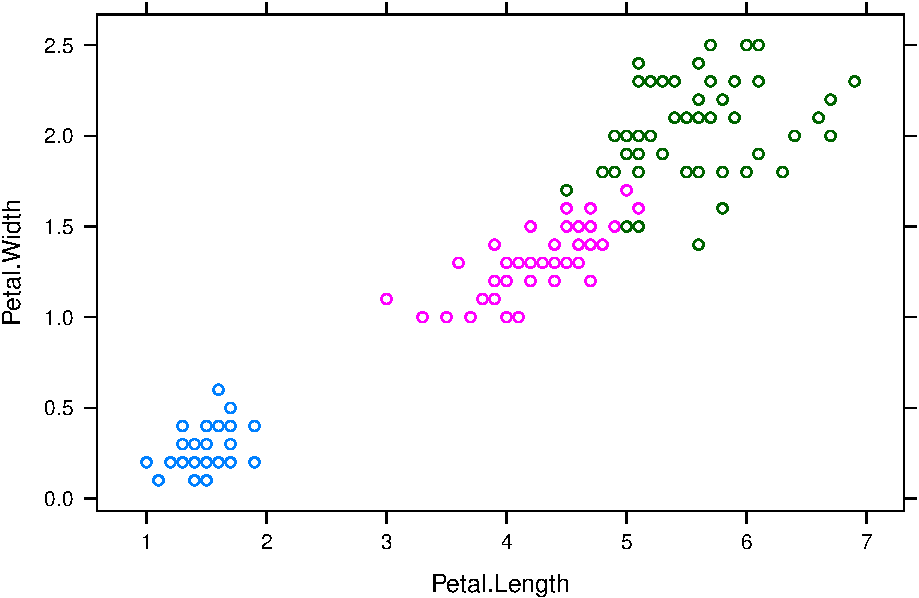
\includegraphics{_main_files/figure-latex/unnamed-chunk-66-1.pdf}
\caption{\label{fig:unnamed-chunk-66}\small Scatterplot of Petal width versus length in the
\texttt{iris} data.}
\end{figure}




\begin{itemize}
\item
  Scatterplot matrices
\item
  splom( \textasciitilde{}
  cbind(GNP.deflator,GNP,Unemployed,Armed.Forces,Population,Year,Employed),
  data = longley)
\item
  splom( \textasciitilde{} cbind(pop15,pop75,dpi), data =
  LifeCycleSavings)
\item
  splom( \textasciitilde{} cbind(Murder, Assault, Rape), data =
  USArrests)
\item
  splom( \textasciitilde{} cbind(CONT, INTG, DMNR), data =
  USJudgeRatings)
\item
  splom( \textasciitilde{} cbind(area,peri,shape,perm), data = rock)
\item
  splom( \textasciitilde{} cbind(Air.Flow, Water.Temp, Acid.Conc.,
  stack.loss), data = stackloss)
\item
  splom( \textasciitilde{}
  cbind(Fertility,Agriculture,Examination,Education,Catholic,Infant.Mortality),
  data = swiss)
\item
  splom(\textasciitilde{} cbind(Fertility,Agriculture,Examination), data
  = swiss) (positive and negative)
\item
  Dot charts
\item
  dotchart(USPersonalExpenditure)
\item
  dotchart(t(USPersonalExpenditure))
\item
  dotchart(WorldPhones) (transpose is no good)
\item
  freeny.x is no good, neither is volcano
\item
  dotchart(UCBAdmissions\{{[}\},,1\{{]}\})
\item
  dotplot(Survived \textasciitilde{} Freq \textbar{} Class, groups =
  Sex, data = B)
\item
  dotplot(Admit \textasciitilde{} Freq \textbar{} Dept, groups = Gender,
  data = C)
\item
  Mosaic plot
\item
  mosaic( \textasciitilde{} Survived + Class + Age + Sex, data =
  Titanic) (or just mosaic(Titanic))
\item
  mosaic( \textasciitilde{} Admit + Dept + Gender, data = UCBAdmissions)
\item
  Spine plots
\item
  spineplot(xtabs(Freq \textasciitilde{} Admit + Gender, data =
  UCBAdmissions))
\item
  rescaled barplot
\item
  Quantile-quantile plots: There are two ways to do this. One way is to
  compare two independent samples (of the same size). qqplot(x,y).
  Another way is to compare the sample quantiles of one variable to the
  theoretical quantiles of another distribution.
\end{itemize}

Given two samples \(x_{1}\), \(x_{2}\), \ldots{}, \(x_{n}\), and
\(y_{1}\), \(y_{2}\), \ldots{}, \(y_{n}\), we may find the order
statistics \(x_{(1)}\leq x_{(2)}\leq\cdots\leq x_{(n)}\) and
\(y_{(1)}\leq y_{(2)}\leq\cdots\leq y_{(n)}\). Next, plot the \(n\)
points \((x_{(1)},y_{(1)})\), \((x_{(2)},y_{(2)})\), \ldots{},
\((x_{(n)},y_{(n)})\).

It is clear that if \(x_{(k)}=y_{(k)}\) for all \(k=1,2,\ldots,n\), then
we will have a straight line. It is also clear that in the real world, a
straight line is NEVER observed, and instead we have a scatterplot that
hopefully had a general linear trend. What do the rules tell us?

\begin{itemize}
\tightlist
\item
  If the \(y\)-intercept of the line is greater (less) than zero, then
  the center of the \(Y\) data is greater (less) than the center of the
  \(X\) data.
\item
  If the slope of the line is greater (less) than one, then the spread
  of the \(Y\) data is greater (less) than the spread of the \(X\) data.
\end{itemize}

\subsection{Lattice Graphics}\label{sub-lattice-graphics}

The following types of plots are useful when there is one variable of
interest and there is a factor in the data set by which the variable is
categorized.

It is sometimes nice to set
\texttt{lattice.options(default.theme\ =\ "col.whitebg")}

\subsubsection{Side by side boxplots}\label{side-by-side-boxplots}

\begin{Shaded}
\begin{Highlighting}[]
\KeywordTok{bwplot}\NormalTok{(~weight |}\StringTok{ }\NormalTok{feed, }\DataTypeTok{data =} \NormalTok{chickwts)}
\end{Highlighting}
\end{Shaded}

\begin{figure}[htbp]
\centering
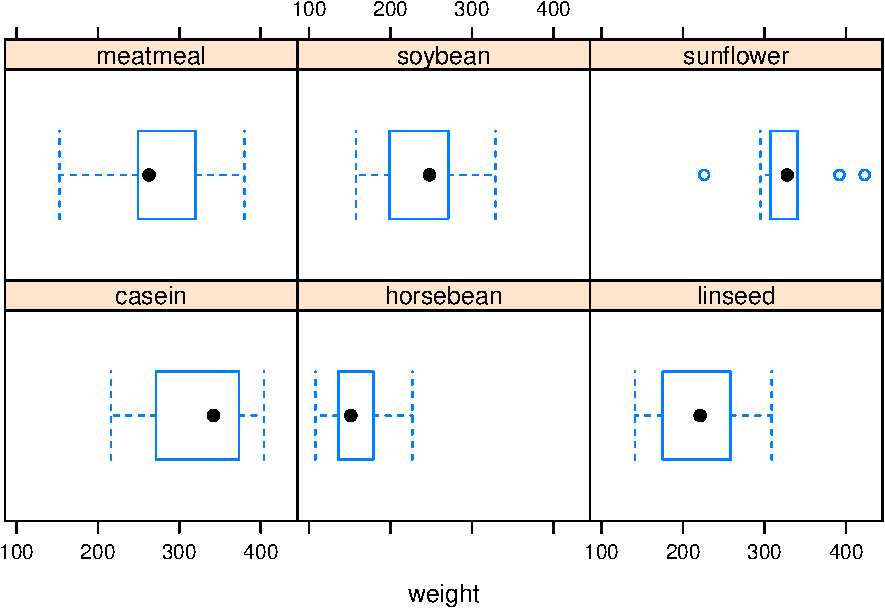
\includegraphics{_main_files/figure-latex/unnamed-chunk-68-1.pdf}
\caption{\label{fig:unnamed-chunk-68}\small Boxplots of \texttt{weight} by \texttt{feed}
type in the \texttt{chickwts} data.}
\end{figure}




\subsubsection{Histograms}\label{histograms}

\begin{Shaded}
\begin{Highlighting}[]
\KeywordTok{histogram}\NormalTok{(~age |}\StringTok{ }\NormalTok{education, }\DataTypeTok{data =} \NormalTok{infert)}
\end{Highlighting}
\end{Shaded}

\begin{figure}[htbp]
\centering
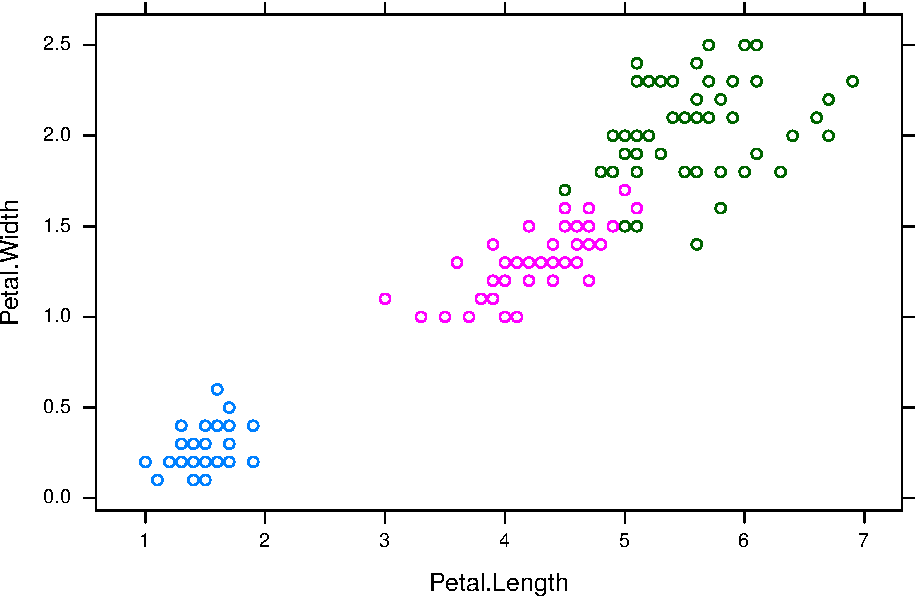
\includegraphics{_main_files/figure-latex/unnamed-chunk-70-1.pdf}
\caption{\label{fig:unnamed-chunk-70}\small Histograms of \texttt{age} by \texttt{education}
level from the \texttt{infert} data.}
\end{figure}




\subsubsection{Scatterplots}\label{scatterplots}

\begin{Shaded}
\begin{Highlighting}[]
\KeywordTok{xyplot}\NormalTok{(Petal.Length ~}\StringTok{ }\NormalTok{Petal.Width |}\StringTok{ }\NormalTok{Species, }\DataTypeTok{data =} \NormalTok{iris)}
\end{Highlighting}
\end{Shaded}

\begin{figure}[htbp]
\centering
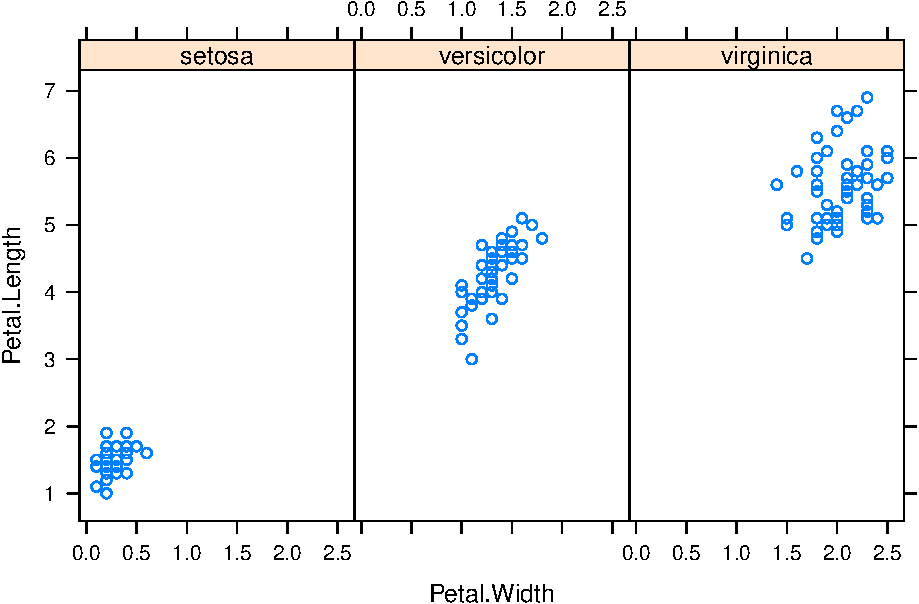
\includegraphics{_main_files/figure-latex/unnamed-chunk-72-1.pdf}
\caption{\label{fig:unnamed-chunk-72}\small An \texttt{xyplot} of \texttt{Petal.Length}
versus \texttt{Petal.Width} by \texttt{Species} in the \texttt{iris}
data.}
\end{figure}





\subsubsection{Coplots}\label{coplots}

\begin{Shaded}
\begin{Highlighting}[]
\KeywordTok{coplot}\NormalTok{(conc ~}\StringTok{ }\NormalTok{uptake |}\StringTok{ }\NormalTok{Type *}\StringTok{ }\NormalTok{Treatment, }\DataTypeTok{data =} \NormalTok{CO2)}
\end{Highlighting}
\end{Shaded}

\begin{figure}[htbp]
\centering
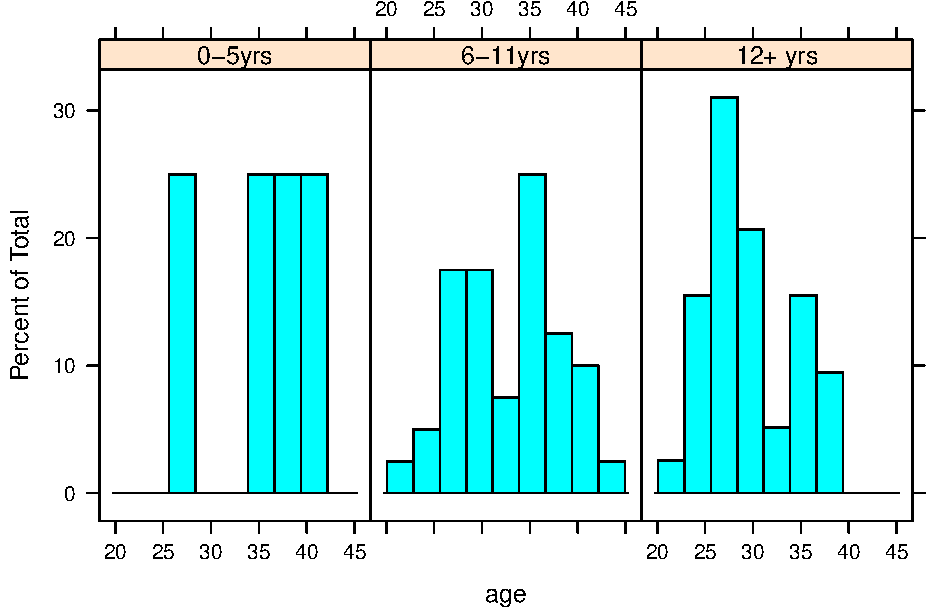
\includegraphics{_main_files/figure-latex/unnamed-chunk-74-1.pdf}
\caption{\label{fig:unnamed-chunk-74}\small A \texttt{coplot} of \texttt{conc} versus
\texttt{uptake} by \texttt{Type} and \texttt{Treatment}.}
\end{figure}

\begin{verbatim}
NULL
\end{verbatim}




\section{Some Remarks about Plotting}\label{some-remarks-about-plotting}

Getting your labels to look right

\begin{Shaded}
\begin{Highlighting}[]
\KeywordTok{library}\NormalTok{(ggplot2)}
\NormalTok{a <-}\StringTok{ }\KeywordTok{qplot}\NormalTok{(state.division, }\DataTypeTok{geom =} \StringTok{"bar"}\NormalTok{)}
\NormalTok{a +}\StringTok{ }\KeywordTok{opts}\NormalTok{(}\DataTypeTok{axis.text.x =} \KeywordTok{theme_text}\NormalTok{(}\DataTypeTok{angle =} \NormalTok{-}\DecValTok{90}\NormalTok{, }\DataTypeTok{hjust =} \DecValTok{0}\NormalTok{))}
\end{Highlighting}
\end{Shaded}

\begin{Shaded}
\begin{Highlighting}[]
\KeywordTok{hist}\NormalTok{(precip, }\DataTypeTok{freq =} \OtherTok{FALSE}\NormalTok{)}
\KeywordTok{lines}\NormalTok{(}\KeywordTok{density}\NormalTok{(precip))}
\KeywordTok{qplot}\NormalTok{(precip, }\DataTypeTok{geom =} \StringTok{"density"}\NormalTok{)}
\NormalTok{m <-}\StringTok{ }\KeywordTok{ggplot}\NormalTok{(}\KeywordTok{as.data.frame}\NormalTok{(precip), }\KeywordTok{aes}\NormalTok{(}\DataTypeTok{x =} \NormalTok{precip))}
\NormalTok{m +}\StringTok{ }\KeywordTok{geom_histogram}\NormalTok{()}
\NormalTok{m +}\StringTok{ }\KeywordTok{geom_histogram}\NormalTok{(}\KeywordTok{aes}\NormalTok{(}\DataTypeTok{y =} \NormalTok{..density..)) +}\StringTok{ }\KeywordTok{geom_density}\NormalTok{()}
\end{Highlighting}
\end{Shaded}

\section{Exercises}\label{exercises-1}

Open R and issue the following commands at the command line to get
started. Note that you need to have the \texttt{RcmdrPlugin.IPSUR}
package \autocite{RcmdrPlugin.IPSUR} installed, and for some exercises
you need the \texttt{e1071} package \autocite{e1071}.

\begin{Shaded}
\begin{Highlighting}[]
\KeywordTok{library}\NormalTok{(}\StringTok{"RcmdrPlugin.IPSUR"}\NormalTok{)}
\KeywordTok{data}\NormalTok{(RcmdrTestDrive)}
\KeywordTok{attach}\NormalTok{(RcmdrTestDrive)}
\KeywordTok{names}\NormalTok{(RcmdrTestDrive)}
\end{Highlighting}
\end{Shaded}

To load the data in the R Commander (\texttt{Rcmdr}), click the
\texttt{Data\ Set} button, and select \texttt{RcmdrTestDrive} as the
active data set. To learn more about the data set and where it comes
from, type \texttt{?RcmdrTestDrive} at the command line.

\textbf{Exercise.} \textless{}\textgreater{} Perform a summary of all
variables in \texttt{RcmdrTestDrive}. You can do this with the command
\texttt{summary(RcmdrTestDrive)}.

Alternatively, you can do this in the \texttt{Rcmdr} with the sequence
\texttt{Statistics} \(\triangleright\) \texttt{Summaries}
\(\triangleright\) \texttt{Active\ Data\ Set}. Report the values of the
summary statistics for each variable.

\textbf{Exercise.} Make a table of the \texttt{race} variable. Do this
with \texttt{Statistics} \(\triangleright\) \texttt{Summaries}
\(\triangleright\) \texttt{Frequency\ Distributions\ -\ IPSUR...} 1.
Which ethnicity has the highest frequency? 1. Which ethnicity has the
lowest frequency? 1. Include a bar graph of \texttt{race}. Do this with
\texttt{Graphs} \(\triangleright\) \texttt{IPSUR\ -\ Bar\ Graph...}

\textbf{Exercise.} Calculate the average \texttt{salary} by the factor
\texttt{gender}. Do this with \texttt{Statistics} \(\triangleright\)
\texttt{Summaries} \(\triangleright\) \texttt{Table\ of\ Statistics...}
1. Which \texttt{gender} has the highest mean \texttt{salary}? 1. Report
the highest mean \texttt{salary}. 1. Compare the spreads for the genders
by calculating the standard deviation of \texttt{salary} by
\texttt{gender}. Which \texttt{gender} has the biggest standard
deviation? 1. Make boxplots of \texttt{salary} by \texttt{gender} with
the following method: \#+BEGIN\_quote On the \texttt{Rcmdr}, click
\texttt{Graphs} \(\triangleright\) \texttt{IPSUR\ -\ Boxplot...} In the
\texttt{Variable} box, select \texttt{salary}. Click the
\texttt{Plot\ by\ groups...} box and select \texttt{gender}. Click
\texttt{OK}. Click \texttt{OK} to graph the boxplot. \#+END\_quote How
does the boxplot compare to your answers to (1) and (3)?

\textbf{Exercise.} For this problem we will study the variable
\texttt{reduction}. 1. Find the order statistics and store them in a
vector \texttt{x}. \emph{Hint:}
\texttt{x\ \textless{}-\ sort(reduction)} 1. Find \(x_{(137)}\), the
137\(^{\mathrm{th}}\) order statistic. 1. Find the IQR. 1. Find the Five
Number Summary (5NS). 1. Use the 5NS to calculate what the width of a
boxplot of \texttt{reduction} would be. 1. Compare your answers (3) and
(5). Are they the same? If not, are they close? 1. Make a boxplot of
\texttt{reduction}, and include the boxplot in your report. You can do
this with the \texttt{boxplot} function, or in \texttt{Rcmdr} with
\texttt{Graphs} \(\triangleright\) \texttt{IPSUR\ -\ Boxplot...} 1. Are
there any potential/suspected outliers? If so, list their values.
\emph{Hint:} use your answer to (a). 1. Using the rules discussed in the
text, classify answers to (8), if any, as \emph{potential} or
\emph{suspected} outliers.

\textbf{Exercise.} In this problem we will compare the variables
\texttt{before} and \texttt{after}. Don't forget
\texttt{library("e1071")}. 1. Examine the two measures of center for
both variables. Judging from these measures, which variable has a higher
center? 1. Which measure of center is more appropriate for
\texttt{before}? (You may want to look at a boxplot.) Which measure of
center is more appropriate for \texttt{after}? 1. Based on your answer
to (2), choose an appropriate measure of spread for each variable,
calculate it, and report its value. Which variable has the biggest
spread? (Note that you need to make sure that your measures are on the
same scale.) 1. Calculate and report the skewness and kurtosis for
\texttt{before}. Based on these values, how would you describe the shape
of \texttt{before}? 1. Calculate and report the skewness and kurtosis
for \texttt{after}. Based on these values, how would you describe the
shape of \texttt{after}? 1. Plot histograms of \texttt{before} and
\texttt{after} and compare them to your answers to (4) and (5).

\textbf{Exercise.} Describe the following data sets just as if you were
communicating with an alien, but one who has had a statistics class.
Mention the salient features (data type, important properties, anything
special). Support your answers with the appropriate visual displays and
descriptive statistics. 1. Conversion rates of Euro currencies stored in
\texttt{euro}. 2. State abbreviations stored in \texttt{state.abb}. 3.
Areas of the world's landmasses stored in \texttt{islands}. 4. Areas of
the 50 United States stored in \texttt{state.area}. 5. Region of the 50
United States stored in \texttt{state.region}.

\printbibliography

\cleardoublepage
\phantomsection
\addcontentsline{toc}{chapter}{\bibname}
%\bibliographystyle{plainurl}
\nocite{*}
%\bibliography{IPSUR,Rpackages}
\vfill{}
\cleardoublepage
\phantomsection
\addcontentsline{toc}{chapter}{\indexname} 
\printindex{}


\end{document}
